% !TeX encoding = UTF-8
% !TeX spellcheck = en_US

%% https://en.wikibooks.org/wiki/LaTeX/Document_Structure
\documentclass[]{clmthesis}

%% https://en.wikibooks.org/wiki/LaTeX/Modular_Documents
% !TeX root = ../mthesis.tex
% !TeX encoding = UTF-8
% !TeX spellcheck = en_US


%% == LaTeX ============================================================= %%
%% https://en.wikibooks.org/wiki/LaTeX
%% ====================================================================== %%


%% -- 2.4 Colors -------------------------------------------------------- %%
%% https://en.wikibooks.org/wiki/LaTeX/Colors
\usepackage[usenames,dvipsnames,svgnames,table]{xcolor}
\input{PREAMBLE/Colors.tex}
%% ---------------------------------------------------------------------- %%


%% -- 2.8 Internationalization ------------------------------------------ %%
%% https://en.wikibooks.org/wiki/LaTeX/Internationalization
\usepackage[utf8x]{inputenc} 		% input
\usepackage[LGR,T1]{fontenc}	 	% output (PDF)
\usepackage[english]{babel}			% language

%% ---------------------------------------------------------------------- %%


%% -- 2.10 Tables ------------------------------------------------------- %%
% https://en.wikibooks.org/wiki/LaTeX/Tables
%% ---------------------------------------------------------------------- %%


%% -- 2.16-17 Hyperlinks ------------------------------------------------ %%
% https://en.wikibooks.org/wiki/LaTeX/Hyperlinks
% https://en.wikibooks.org/wiki/LaTeX/Labels_and_Cross-referencing
\usepackage{hyperref}
%\usepackage[xindy,toc]{glossaries}
\usepackage[toc]{glossaries}
\usepackage[]{index}
%% ---------------------------------------------------------------------- %%


%% -- 4.1-3 Mathematics ------------------------------------------------- %%
% https://en.wikibooks.org/wiki/LaTeX/Mathematics
% https://en.wikibooks.org/wiki/LaTeX/Advanced_Mathematics
\usepackage{amsmath}
\usepackage{mathtools}
\usepackage{amssymb}

% https://en.wikibooks.org/wiki/LaTeX/Theorems
\usepackage{amsthm}
\usepackage{proof}
\usepackage{bussproofs}
\usepackage{marvosym}

\usepackage{multirow}
\usepackage[makeroom]{cancel} % \(b|x)cancel(to{}){}
\usepackage{soul}
\usepackage{pdfcomment}


%% ---------------------------------------------------------------------- %%


\usepackage{varioref}


%\usepackage{calc}
%\usepackage{geometry}

%% -- 4.5 Algorithms ---------------------------------------------------- %%
% https://en.wikibooks.org/wiki/LaTeX/Algorithms
%% ---------------------------------------------------------------------- %%


%% -- 4.6 Listings ------------------------------------------------------ %%
% https://en.wikibooks.org/wiki/LaTeX/Source_Code_Listings
\usepackage{listings}
\input{PREAMBLE/Listings.tex}	% definitions
%% ---------------------------------------------------------------------- %%


%% -- Graphics ---------------------------------------------------------- %%
% https://en.wikibooks.org/wiki/LaTeX/PGF/TikZ
\usepackage{tikz}
\documentclass{clseminar}

    \usepackage{tikz}

    % \documentclass{clseminar}

    \usepackage{tikz}

    % \input{../PREAMBLE/Drawings}

\begin{document}

\begin{figure}
\input{../DRAWINGS/ProperOrder}
\caption{Proper orders on terms}
\end{figure}

\begin{figure}
\input{../DRAWINGS/PartialOrder}
\end{figure}

\end{document}

\begin{document}

\begin{figure}
\begin{tikzpicture}
    \node (defCUC) at (-4,8.5) { $s\succ t\Rightarrow C[s]\succ C[t]$};
    \node (CUC) at (-4,8) { contexts };
    \node (defCUS) at (0,8.5) { $s\succ t\Rightarrow s\sigma\succ t\sigma$};
    \node (CUS) at (0,8) { substitutions };

        \node (CL) at (-2,6) { closed under };
        \node (defIRR) at (2,6.5) { $s\not>s$ };
        \node (IRR) at (6,6) { irreflexive };
        \node (defIRR) at (6,6.5) { $s>t>u\Rightarrow s>u$ };
        \node (TRA) at (2,6) { transitive };

        \node (PO) at (4,4.4) { $>$ };
        \node (PO) at (4,4) { proper order };
        \node (RWR) at (0,4) { rewrite relation };

        \node (defSTP) at (-2,2.5) { $C[s]\succ s$ };
        \node (STP) at (-2,2) { subterm property };
        \node (RWO) at (2,2) { rewrite order };
        \node (defWF) at (8,4.5) { $(s_i Rs_{i+1})_i$ is finite };
        \node (WF) at (8,4) { well-founded };

        \node (SO) at (0,0) {simplification order};
        \node (RO) at (4,0) {reduction order};

        \node (WFO) at (6,2) { well-founded order };


        \draw[->] (CL) -- (CUC);
        \draw[->] (CL) -- (CUS);

        \draw[->] (PO) -- (IRR);
        \draw[->] (PO) -- (TRA);π

        \draw[->] (RWR) -- (CL);

        \draw[->] (RWO) -- (PO);
        \draw[->] (RWO) -- (RWR);

        \draw[->] (SO) -- (STP);
        \draw[->] (RO) -- (RWO);
        \draw[->] (RO) -- (WFO);
        % \draw (RO) edge[out=0,in=-45,->] (WF);

        \draw[->] (SO) -- (RWO);
        \draw[->, dotted] (SO) -- (RO);

        \draw[->] (WFO) -- (WF);
        \draw[->] (WFO) -- (PO);

        \draw[->, dotted] (WF) -- (IRR);


    \end{tikzpicture}
\caption{Proper orders on terms}
\end{figure}

\begin{figure}
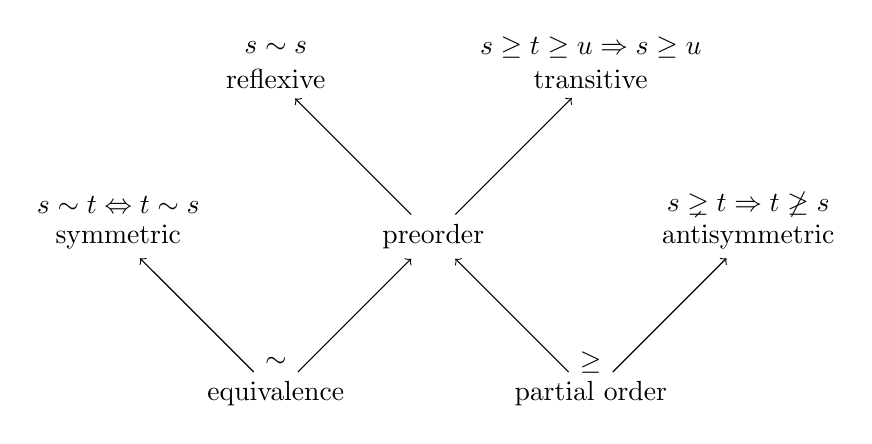
\begin{tikzpicture}

        \node (defSYMMETRIC) at (-4,0.4) { \( s\sim t\Leftrightarrow t\sim s \) };
        \node (SYMMETRIC) at (-4,0) { symmetric };

            \node (defREFLEXIVE) at (-2,2.4) { \( s\sim s \) };
            \node (REFLEXIVE) at (-2,2) { reflexive };

                \node (defTRANSITIVE) at (2,2.4) { \( s\geq t\geq u\Rightarrow s\geq u \) };
                \node (TRANSITIVE) at (2,2) { transitive };

                    \node (defANTISYMMETRIC) at (4,0.4) { \( s\gneq t \Rightarrow t\not\geq s \) };
                    \node (ANTISYMMETRIC) at (4,0) { antisymmetric };

        \node (PREORDER) at (0,0) { preorder };

    \node (SIM) at (-2,-1.6) { \( \sim \) };
    \node (EQUIVALENCE) at (-2,-2) { equivalence };

    \node (GEQ) at (2,-1.6) { \( \geq \) };
    \node (PARTIAL) at (2,-2) { partial order };

    % \node (PROPER) at (5,-1.5) { proper order };

    \draw[->] (PREORDER) -- (REFLEXIVE);
    \draw[->] (PREORDER) -- (TRANSITIVE);

    \draw[->] (EQUIVALENCE) -- (SYMMETRIC);
    \draw[->] (EQUIVALENCE) -- (PREORDER);
    \draw[->] (PARTIAL) -- (PREORDER);
    \draw[->] (PARTIAL) -- (ANTISYMMETRIC);

    % \draw[->] (PROPER) -- (TRANSITIVE);
\end{tikzpicture}
\end{figure}

\end{document}		% definitions and tikz macros
\usepackage[thinlines,thiklines]{easybmat}
%% ---------------------------------------------------------------------- %%

%% -- Macros ------------------------------------------------------------ %%
%% https://en.wikibooks.org/wiki/LaTeX/Macros
\usepackage{xspace}
% !TeX encoding = UTF-8

%% ==============================================================
%% ### MY MATH ENVIRONMENTS ###

\theoremstyle{plain}
%\newtheorem{theorem}{Theorem}			% predefined in CL?
%\newtheorem{proposition}{Proposition}	% predefined in CL?
%\newtheorem{lemma}{Lemma}				% predefined in CL?
%\newtheorem*{corollary}{Corollary}		% predefined in CL?

\theoremstyle{definition}
%\newtheorem{definition}{Definition}	% predefined in CL?
\newtheorem{conjecture}{Conjecture}
%\newtheorem*{example}{Example}			% predefined in CL?
%\newtheorem{algorithm}{Algorithm}		% predefined in CL
\newtheorem{procedure}{Procedure}
\newtheorem{goal}{Goal}
\newtheorem{notation}{Notation}

\theoremstyle{remark}
\newtheorem*{remark}{Remark}			% predefined in CL?
\newtheorem*{observation}{Observation}
%\newtheorem*{note}{Note}
%\newtheorem{case}{Case}

%% ==============================================================
%% ### MY MATH DEFINITIONS ###

% math alphabets

\DeclareMathAlphabet{\mathpzc}{OT1}{pzc}{m}{it}	% \mathpzc
\DeclareMathAlphabet{\mathcll}{T1}{calligra}{m}{n}

% math operators

\DeclareMathOperator{\arity}{arity}		% arity of a symbol

\DeclareMathOperator{\var}{\mathpzc{Vars}}			% variables of a term
\DeclareMathOperator{\fun}{\mathpzc{Funs}}			% function symbols of a term
\DeclareMathOperator{\pos}{\mathpzc{Pos}}			% positions in a term
\DeclareMathOperator{\posT}{\mathpzc{{t-}Pos}}			% positions in a term
\DeclareMathOperator{\posS}{\mathpzc{Pos^F}}
\DeclareMathOperator{\fvar}{\mathpzc{Fvars}}
\DeclareMathOperator{\bvar}{\mathpzc{Bvars}}

\DeclareMathOperator{\domain}{dom}			% domain of an assignment
\DeclareMathOperator{\range}{rng}		% range of an assignment
\DeclareMathOperator{\image}{img}			% image of an assignment

\DeclareMathOperator{\mgu}{mgu}			% most general unifier
\DeclareMathOperator{\sel}{sel}			% selection function

%\DeclareMathOperator{\mul}{mul}
%\DeclareMathOperator{\add}{add}
\DeclareMathOperator{\head}{head}
\DeclareMathOperator{\tail}{tail}
\DeclareMathOperator{\length}{length}



\DeclareMathOperator{\UNIF}{unifiable}
\DeclareMathOperator{\INST}{instance}
\DeclareMathOperator{\GNRL}{generalization}
\DeclareMathOperator{\VRNT}{variant}
\DeclareMathOperator{\PSTR}{pstr}

%\DeclareMathOperator{\subterms}{\mathpzc{Subterms}}	
%\DeclareMathOperator{\termsize}{size}
%\DeclareMathOperator{\symbols}{symbols}
%\DeclareMathOperator{\subforms}{\mathpzc{Subforms}}	
% !TeX encoding = UTF-8

% shortens the definition by cases
\newcommand{\DEFINE}[3][=]{{
		\begin{gather*}
		#2 #1 \left \{
				\begin{array}{ll}
					#3
				\end{array}
		\right.
		\end{gather*}
	}}


% accepts greek as input
\newcommand{\textgreek}[1]{\begingroup\fontencoding{LGR}\selectfont#1\endgroup}

\newcommand{\tikzmark}[1]{\tikz[overlay,remember picture] \node (#1) {};}


		% complex macros
\documentclass[]{clseminar}

    \documentclass[]{clseminar}

    \input{../PREAMBLE/Symbols}
    
    \begin{document}
    
    \author{Alexander Maringele}
    \title{Symbols}
    \abstract{The quick brown fox jumps over the lazy dog.
    Why?}
    
    \maketitle

    \newcommand{\demo}[1]{$#1$}

    \begin{itemize}
        \item \verb+\myem+ \myem The quick brown fox jumps over the lazy dog
        \item 
        \demo{\disjointunion},,
        \verb+\disjointunion+ 
        $\disjointunion$, 
        \verb+\false+ 
        $\false$,
        \verb+\lbic+ 
        $\lbic$,  
        \verb+\limp+ 
        $\limp$,  
        \verb+\succG\succL\succC+
        $\succG$,   
        \verb+\succG\succL\succC+
        $\succL$,   
        \verb+\succG\succL\succC+
        $\succC$, 
        \verb+\true+ $\true$

    \end{itemize}



    
        
    \end{document}
    
    \begin{document}
    
    \author{Alexander Maringele}
    \title{Symbols}
    \abstract{The quick brown fox jumps over the lazy dog.
    Why?}
    
    \maketitle

    \newcommand{\demo}[1]{$#1$}

    \begin{itemize}
        \item \verb+\myem+ \myem The quick brown fox jumps over the lazy dog
        \item 
        \demo{\disjointunion},,
        \verb+\disjointunion+ 
        $\disjointunion$, 
        \verb+\false+ 
        $\false$,
        \verb+\lbic+ 
        $\lbic$,  
        \verb+\limp+ 
        $\limp$,  
        \verb+\succG\succL\succC+
        $\succG$,   
        \verb+\succG\succL\succC+
        $\succL$,   
        \verb+\succG\succL\succC+
        $\succC$, 
        \verb+\true+ $\true$

    \end{itemize}



    
        
    \end{document}			% simple macros
%% ---------------------------------------------------------------------- %%

\usepackage{epigraph}


	% \usepackage{mystyle}	

\includeonly{
%	introduction/introduction,
	preliminaries/preliminaries,
%	proving/proving,
%	epr/epr,
%	flea/flea,
%	conclusion/conclusion,
%	appendix/main
}

\begin{document}
% \nocite{*}

% BEGIN: titlepage setup -------------------------------------------
\title{Yet another first order theorem prover with equality}
\plaintitle{Theorem prover with equality}
\mailaddress{alexander.maringele@uibk.ac.at}
\matriculationnumber{8517725}
\author{Alexander~Maringele}
\plainauthor{Alexander~Maringele}
\date{\today}
\supervisor{Assoc.~Prof.~Dr.~Georg~Moser}
\institute{Institute of Computer Science}

\abstract{Instantiation-based ...}
% END: titlepage setup ----------------------------------------------


%\acknowledgments{Thanks.}
%\maketitle
\tableofcontents

%====================================================================
% BEGIN: CONTENT ----------------------------------------------------
%====================================================================

\include{introduction/introduction}
% !TeX root = ../mthesis.tex
% !TeX encoding = UTF-8
% !TeX spellcheck = en_US

\chapter{Preliminaries}





\epigraph{
	A good theory starts 
	
	with a good definition
}{
	unknown
}

We assume familiarity with propositional and predicate logic \cite{Huth:2004:LCS:975331}, 
automated theorem proving \cite{Fitting:1996:FLA:230183}, 
term rewriting \cite{Baader:1998:TR:280474}, 
decision procedures \cite{Kroening:2008:DPA:1391237}, 
and (maximum) satisfiability testing \cite{Biere:2009:HSV:1550723}.
Even so, for clarity we introduce basic
definitions and state basic lemmas and theorems without proofs.
This section is an extension of the same section in our seminar report \cite{axm:SR2}
where notions and notations largely follow those in lecture notes \cite{AM2015tr} and \cite{GM2013ar}.


\section{Syntax}

% !TeX root = ../mthesis.tex
% !TeX encoding = UTF-8
% !TeX spellcheck = en_US

\begin{definition}\label{def:signature}
A
first order
{\myem signature} with equality
%with equality
$\mcF = \mcFfPE$
is the disjoint union of
a set of {\myem function symbols} $\mcFf$,
a set of {\myem predicate symbols} $\mcFP$,
and one distinct equality symbol.
%
The {\myem arity} of a symbol determines the number of its arguments in a first order expression.
With $\mcFn = \{ \mcf\in\mcF \mid \arity(\mcf) = n \}$ we denote symbols with arity $n$.
\end{definition}

\begin{remark}
    We use $\mEQ$ as equality symbol in our signatures to emphasize
    that at this point it is just a highlighted symbol
    without “meaning”.
    On the other hand we use $=$ to express “identity” of objects
    like formualae or sets
    without actually defining how this identity can be determined.
\end{remark}


% !TeX root = ../mthesis.tex
% !TeX encoding = UTF-8
% !TeX spellcheck = en_US

\begin{definition}
	We build the set of (function) {\myem terms} $\mcTfFV$ 
	from function symbols $\mcFf \subseteq \mcF$ and 
	a countable set of {\myem variables} $\mcV$ disjoint from $\mcF$.
	Every variable $x\in\mcV$ is a term,
	every constant $c\in\mcFf^{(0)}$ is a term, 
	and every expression $f(t_1,\ldots,t_n)$
	for every function symbol $f\in\mcFf$ 
	with arity $n>0$ 
	and terms $t_1,\ldots,t_n$
	is a term.
%	
	We build the set of predicate terms or {\myem atoms} $\mcTPFV$
	from predicate symbols $\mcFP \subseteq \mcF$ and terms $t\in\mcTfFV$. 
	Every proposition $p\in\mcFP^{(0)}$ is an atom 
	and every expression $P(t_1,\ldots,t_n)$
	for every predicate symbol $P\in\mcFP$ with arity $n>0$ and terms $t_1,\ldots,t_n$ is an atom.
%	Every equation $s\ \mEQ\ t$ for terms $s,t$ is an atom too.
%
%	We speak of the set of general terms 
%	$\mcTFV = \mcTfFV\disjointunion\mcTPFV$ as the disjoint union of terms and atoms.
\end{definition}



% !TeX root = ../mthesis.tex
% !TeX encoding = UTF-8
% !TeX spellcheck = en_US

\begin{definition}\label{def:predicates}\label{def:equations}\label{def:atoms}
	We build the set of (first order) {\myem predicates} $\mcPT$
	from predicate symbols and terms.
	Every proposition $\mpp\in \mcFPn[0]$ is a predicate,
	and every expression $\mP(t_1,\ldots,t_n)$ is a predicate for $n>0$,
	predicate symbol $\mP\in\mcFPn$ and arbitrary terms $t_1,\ldots,t_n$.
%
	We build the set of (first order) {\myem equations }$\mcET$ from the equality symbol and terms.
	Every pair $s\mEQ t$ is an equation %\footnote{
%		We use prefix and infix notation interchangeable,
%		e.g.~${\mEQ}(s,t)$ represents the same equation as $s\mEQ t$.}
	for arbitrary terms $s$ and $t$.
%
	The set of atomic formulas (or {\myem atoms} for short) is the (distinct) union of predicates and equations.
\end{definition}

\input{preliminaries/ground}

% !TeX root = ../mthesis.tex
% !TeX encoding = UTF-8
% !TeX spellcheck = en_US

\begin{definition}[\index{FOF}\FOF]\label{def:syntax:FOF}
	Atoms from the previous definition are {\myem first order formulae}.  
	The universal quantification $(\forall x F)$ 
	and the existential quantification $(\exists x F)$ 
	of a first order formula are (quantified) first order formulae
	with {\myem bound} variable $x\in\mcV$.
	The negation $(\lnot F)$ of a first order formula
	is a (composite) first order formula.
	Further, the disjunction $(F \lor F')$, 
	the conjunction $(F \land F') $, 
	and the implication $(F \limp F')$ 
	of two first order formulae
	are (composite) first order formulae.
\end{definition}

\begin{definition}\label{def:term:vars}\label{def:fof:fvars}\label{def:fof:sentence}
	We define the set of variables of a first order term $t$ and the set of {\myem free} variables of a first order formula $F$ as follows:
\DEFINE{\var(t)} {
		\{ x \} & \text{if } t = x \in \mcV \\
		\bigcup_{i=1}^n \var(t_i) & \text{if }  t = \mf(t_1, \ldots t_n)
	}
\DEFINE{\fvar(F)}{
		\bigcup_{i=1}^n \var(t_i) &\text{if }F = \mP(t_1,\ldots,t_n)\text{ or }t_1\mEQ t_{n=2} 
		\\
		\fvar (G) \setminus \{ x\} &\text{if } F \in\{\, \forall x\,G, \exists x\,G\,\}
		\\
		\fvar(G) \cup \fvar(H)&\text{if }F \in\{\,G\land H,G\lor H,G\limp H\,\}
%		\\
%		\var(s) \cup \var(t) &\text{if }F = s\mEQ t
		\\
		\fvar(G)&\text{if }F = \lnot G
	}
\end{definition}

\begin{definition}\label{def:fof:closed}
	A closed first order formula or in other words
	a first order {\myem sentence} 
	is a first order formula without free variables,
	i.e.~all occurring variables are bound.
	\DEFINE{\bvar(F)}{
		\emptyset &\text{if }F = \mP(t_1,\ldots,t_n)\text{ or }t_1\mEQ t_{n=2} 
		\\
		\bvar (G) \cup \{ x\} &\text{if } F \in\{\, \forall x\,G, \exists x\,G\,\}
		\\
		\bvar(G) \cup \bvar(H)&\text{if }F \in\{\,G\land H,G\lor H,G\limp H\,\}
		%		\\
		%		\var(s) \cup \var(t) &\text{if }F = s\mEQ t
		\\
		\bvar(G)&\text{if }F = \lnot G
	}
\end{definition}

%\begin{remark} 
	We often will write formulae or sentences 
	without stating the first order signature.
The reader can easily deduce the underlying {\myem implicit} signature with arities 
and the set of variables by applying the definitions of the syntax for first order formulae.
We follow the convention to use $x,y,z$ for variables 
and $\ma,\mb,\mc$ for constant function symbols 
(which avoids ambiguity in the presence of free variables). 
For easier readability we will use uppercase predicate symbols and lowercase function symbols.
%\end{remark}

% !TeX root = ../mthesis.tex
% !TeX encoding = UTF-8
% !TeX spellcheck = en_US

\begin{definition}\label{def:literals}
A {\myem literal} $L$ is either an atom
or the negation of an atom.
%, where $l\not{}\hspace{-0.5mm}\circ$ abbreviates $\lnot(l\circ r)$
%for binary symobl $\circ$.
%A literal is ground if all its terms are ground.
%The complement $L^c$ of a literal $L$ is defined as %with some atom $A$: 
%\[ L^c = \left\{ \begin{array}{rl}
%A & \text{if } L = \lnot A\\
%\lnot A & \text{if } L = A
%\end{array}\right.
%\]
Two literals are complementary if one is an atom and the other is the negation of this atom.
%
A {\myem clause}\ \ $\mcC = L_1\lor\ldots\lor L_n$  is a possible empty multiset of literals 
and is equivalent to the universally quantified disjunction of its literals.
The {\myem empty clause} $\emptyclause$ expresses a contradiction. 
%A clause is ground if all its literals are ground.
A finite {\myem set of clauses} $S=\{ \mcC_1,\ldots,\mcC_n \}$ 
is equivalent to the conjunction of its clauses.
$S\equiv(\forall\vec{x}_1\mcC_1)\land\ldots\land(\forall\vec{x}_n\mcC_n)$ with 
$\vec{x}_i = \var(\mcC_i)$.
%$\vec{x}_i\cap\vec{x}_j=\emptyclause\lor i=j$.
%A set of clauses is ground if all its clauses are ground.
\end{definition}

% !TeX root = ../mthesis.tex
% !TeX encoding = UTF-8
% !TeX spellcheck = en_US

\begin{definition}\label{def:substitution}
	A {\myem substitution} $\sigma$ is a mapping from variables $x\in\mcV$ to terms in $\mcTFfV$
	where the {\myem domain }$\dom(\sigma) = \{ x\in\mcV\mid\sigma(x) \neq x \}$ is finite.
	We write substitutions as bindings $\sigma=\{ x_1\mapsto s_1,\ldots,x_n\mapsto s_n \}$
	where $\dom(\sigma)=\{ x_1,\ldots,x_n \}$ and $\sigma(x_i)=s_i$.
	A {\myem variable substitution} is a mapping from $\mcV$ to $\mcV$.
	A {\myem renaming} is a bijective variable substitution.
	A {\myem proper instantiator} is a substitution that is not a variable substitution.
	We define the instance $\mkt\sigma$ of a term, literal or clause $\mkt$,
	respectively the application of a substitution $\sigma$ to terms, literals, and clauses as follows:
	\begin{align*}
		\mkt\sigma &= \left\{\begin{array}{ll}
			s_i 					& \text{if }T=x_i\in\dom(\sigma)\\
			y					& \text{if }T=y\in\mcV\,\backslash\dom(\sigma)\\
%			c					& \text{if }tc \in \mcFf^{\!0}\\
			f(t_1\sigma,\ldots,t_n\sigma)	&\text{if }T=f(t_1,\ldots,t_n), f\in\mcFfn \\[0.5em]
			P(t_1\sigma,\ldots,t_n\sigma)	&\text{if }T=P(t_1,\ldots,t_n), P\in\mcFPn \\
			s\sigma\mEQ t\sigma			&\text{if }T=s\mEQ t \\[0.5em]
			\lnot(A\sigma)					&\text{if }T=\lnot A \\
			L_1\sigma\lor\ldots\lor L_n\sigma	&\text{if }T=L_1\lor\ldots\lor L_n \\
		\end{array}\right.	
	\end{align*}
%	
	We define the {\myem composition} of two substitutions $\sigma$ and $\tau$ as follows
	\begin{align*}
		\sigma\tau&=\{ x_i\mapsto s_i\tau\mid x_i\in\dom(\sigma) \}
		\cup
		\{ y_i\mapsto t_i\mid y_i\in\dom(\tau) \backslash \dom(\sigma) \}.
	\end{align*}
	
\end{definition}

\begin{lemma}\label{lem:substitution}
	With the definitions in \ref{def:substitution} the identity
%	$(\mkt\sigma)\tau = \mkt(\sigma\tau)$ holds for
	arbitrary terms, literals, clauses, and substitutions.
\end{lemma}

% !TeX root = ../mthesis.tex
% !TeX encoding = UTF-8
% !TeX spellcheck = en_US

\begin{definition}\label{def:unifier}
Two terms $s$ and $t$ are {\myem unifiable} if there exists a substitution $\sigma$ such that $s\sigma=t\sigma$.
They are {\myem variants} if their most general unifier is a renaming.
The {\myem most general unifier} $\sigma=\mgu(s,t)$ is a unifier such that
for every other unifier $\sigma'$ there exists a substitution $\tau$ such that
$\sigma' = \sigma \tau$. 
\end{definition}

\section{Semantics}

In this section we recall some basic aspects and definitions of semantics in first order logic. 
We state satisfiability of clauses. For brevity we ignore arbitrary formulas in first order logic
in our definitions.

\begin{definition}
	An {\myem interpretation} $\mcI$ over a signature $\mcF$ consists of a
	non-empty set $A$ -- the {\myem universe} or {\myem domain},
	definitions of (partial) functions $\mf_\mcI: A^n\rightarrow A$ for every function symbol $\mf\in\mcFf$, 
	and definitions of (possibly empty) n-ary relations 
	 ${\mP_\mcI}\subseteq A^n$ for every predicate symbol $\mP\in\mcFP$
	 and the definition of a binary relation ${\mEQ_\mcI}\subseteq A^2$ for the equality symbol.
	 An {\myem equational} interpretation defines $\mEQ_\mcI$ as equality on its domain.
	 i.e.~a ground term $s \mEQ_\mcI t$ holds if and only if $s_\mcI = t_\mcI$.
	
	A ground predicate $\mP(t_1,\ldots,t_n)$ {\myem holds} in interpretation $\mcI$ 
	if and only if $(t_1,\ldots,t_n) \in \mP_\mcI$.
	A ground literal does not hold in $\mcI$ if and only if its complementary literal holds in $\mcI$.
%	
	A non-ground literal holds in $\mcI$ if all its 
	(perhaps infinitely many) ground
	instances hold in $\mcI$.
	A clause holds in $\mcI$ if at least one of its literals holds in $\mcI$.
	A set of clauses $S$ holds in $\mcI$ if every clause $\mcC\in S$ holds in $\mcI$.
	We say $\mcI$ is a model {\em for} $S$ if $S$ holds in $\mcI$. 
	
	
\end{definition}

\begin{definition}
	A set of clauses $S$ is {\myem satisfiable} if and only if there is a model $\mcM$ for $S$. 
	A set of clauses is  {\myem valid} if and only if all clauses hold in every interpretation.
\end{definition}

\begin{definition}\label{def:hk}
	An {\myem Herbrand universe} is the smallest set of terms that contains all $H_k\ge 0$ of
	\begin{align*}
	H_0 &:= \left\{ 
	\begin{array}{ll}
	\{ \mc \mid \mc\in\mcFfn[0] \} 
	&\text{if } \mcFfn[0]\not=\emptyset\\
	\{ \mc \}
	&\text{if } \mcFfn[0]=\emptyset, \mc\not\in\mcF
	\end{array}
	\right. 
	\\
	H_{k+1} &:= H_k \cup \{\  
	\mf(t_1,\ldots,t_n) \mid
	\mf\in\mcFfn[n],
	t_1,\ldots,t_n \in H_k
	\ \}
	\end{align*}
	
\end{definition}

\begin{definition}
	An {\myem Herbrand interpretation} $\mcH$ is an interpretation where the domain 
	is an Hebrand universe
	and the interpretation of each ground term $t_\mcH := t$ is the term itself.
\end{definition}

\begin{example}
	Consider the satisfiable set of clauses 
	$S = \{  
		\mP(\mf(x)) 
	\}$. 
	Let $H_S = \{ 
		\mc, \mf(\mc), \mf(\mc), \ldots, \mf^i(\mc), \ldots
	\}$ be the Hebrand universe for $S$.
	We define $\mf_I$ by mapping $\mc_I := \mc$,
	$\mf_I^{i+1}(x) := \mf (\mf_I^i(x))$
\end{example}

\begin{definition}
	An {\myem term interpretation} 
	$\mcI_t$ 
	is an interpretation 
	where the elements of its domain $A = \mcTFf/_\sim$ 
		are equivalence classes of ground terms
		and the interpretation of each ground term $t^{\mcI_t} := [t]_\sim$ is its equivalence class.
%		An equation $s\mEQ t$ of ground terms holds in if $[s]_\sim=[t]_\sim$.
	 A ground predicate $\mP(t_1,\ldots,t_n)$ holds if 
	 $([t_1]_\sim,\ldots,[t_n]_\sim) \in \mP^{\mcI_t} \subseteq A^n$.
%	A ground literal does not hold if and only if its complementary literal holds.
	In an {\myem equational} term interpretation an equation $s\mEQ t$ holds if an only if $s\sim t$.
	
\end{definition}

\begin{example}
	Consider the satisfiable set of clauses $S = \{ x \mEQ \mf(x) \}$. 
%	
	We easily find a Herbrand model $\mcH$ with
	predicate definition $\mEQ^\mcH = \{ (\mf^{i}(\ma)), \mf^{i+1}(\ma)) \mid i\geq 0  \} $. 
	However $\mcH$ is not an equational model because obviously $\ma\neq\mf(\ma)$ in its domain.
%	
	Further on we easily find an equational model $\mcM$ 
	with domain $\{ \mc \}$, function definition $\mf^\mcM(\mc) = \mc$, 
	and $\mEQ_\mcM$ is defined by equality in its domain.
	Certainly this model $\mcM$ is not an Hebrand model 
	because the interpretation of ground term ${\mf(\mc)}^\mcM \neq \mf(\mc)$ is not the term itself.
	
	On the other hand we easily get an equational term model with domain $\{ [\ma]_\sim\}$, 
	a plain function definition
	$\mf([\ma]_\sim) = [\ma]_\sim$, 
	and an equivalence relation
	$\ma \sim \mf(\ma)$
	where $\mEQ$ is defined by equality in its domain.	
\end{example}


%\section{Term Rewriting}
%
%
%
%
%\begin{definition}
%	A {\myem rewrite rule} is an equation of terms where the left-hand side is not a variable
%	and the variables occuring in the right-hand side occur also in the left-hand side.
%	%	\[
%	%		\ell\rwEQ r \text{ is rewrite rule }\quad :\Longleftrightarrow\quad\ell\not\in\mcV\text{ and }\var(r)\subseteq\var(l)
%	%	\] 
%	A rewrite rule $\ell'\rwEQ r'$ is a {\myem variant} of $\ell\rwEQ r$ if there is a renaming $\varrho$
%	such that 
%	$(l\rightarrow r)\varrho = l'\rightarrow r'$.
%	A {\myem term rewrite system} is a set of rewrite rules without variants.
%\end{definition}
%
%\begin{definition}\label{def:position}
%	A {\myem position} is a finite sequence of positive integers.
%	The root position is the empty sequence $\epsilon$.
%	The position $pq$ is obtained by concatenation of positions $p$ and $q$.
%	%
%	The set of all positions of an expression $\mct$ is defined as 
%	\DEFINE{ 
%		\pos(\mct) }
%	{
%		\{ \epsilon \} 		
%		& \text{if }\mct = x \in \mcV \\
%%		
%		\{ \epsilon \} \cup \bigcup_{i=1}^{n} \{ iq\mid q\in\pos(t_i) \}	
%		& \text{if }\mct=\mcf(t_1,\ldots,t_n)\text{ where } \mcf\in\mcF^{(n)}.
%	}
%The~{\myem subexpression} $\mct|_p$ of an expression $\mct$ {\myem at position} $p\in\pos(\mct)$ is defined as
%%
%\DEFINE{
%	t|_p
%}{
%	t 		& \text{if }p=\epsilon \\
%	t_i|_q	& \text{if }t=\mcf(t_1,\ldots,t_n)\text{ and }p=iq
%}
%%
%If $s$ is an expression then $t[s]_p$ represents the expression build by replacing the subexpression of $t$ at position $p$ with the term $s$.
%\DEFINE{
%	t[s]_p}
%{
%	s 		& \text{if }p=\epsilon \\
%	\mf(t_1,\ldots,t_i[s]_q,\ldots,t_n)	& \text{if }t=\mf(t_1,\ldots,t_n)\text{ and }p=iq
%}
%%A {\myem hole} denotes a special constant symbol $\ctxhole\in\mcFf^{(0)}$. 
%%A {\myem context} is a term $t$ with exactly one hole, i.e.~one occurrence $|t|_{\ctxhole}=1$.
%\end{definition}
%
%\begin{definition}
%	We say $s\rightarrow_\mcR t$ is a 
%	{\myem rewrite step} 
%	 with respect to TRS $\mcR$ 
%	when there is a position $p \in \pos(s)$, 
%	a rewrite rule $l\rwEQ r\in\mcR$, 
%	and a substitution $\sigma$ such that
%	$s|_p=l\sigma$ and $s[r\sigma]_p = t$.
%		The subterm $l\sigma$ is called {\myem redex} and
%	$s$ rewrites to $t$ by {\myem contracting} $l\sigma$ to {\myem contractum} $r\sigma$.
%	%
%	We say a term $s$ is {\myem irreducible} or in {\myem normal form} with respect to TRS $\mcR$ if there is no rewrite step $s\rightarrow_\mcR t$ for any term $t$. 
%	The set of normal forms $\mNFR$ contains all irreducible terms of the TRS $\mcR$.
%	\end{definition}
%
%%\begin{definition}
%%	A {\myem rewrite relation} is a binary relation on terms that is closed under contexts and substitutions.
%%	A {\myem rewrite order} is a proper order (i.e. irreflexive and transitive relation) and a rewrite relation.
%%	A {\myem reduction order} is a well-founded rewrite order.
%%\end{definition}
%
%\begin{definition}
%	A term $s$ can be rewritten to term $t$ with notion $s\rightarrow^*_\mcR t$ 
%	if there exists at least one {\myem rewrite sequence} $(a_1,\ldots ,a_n)$ such that
%	$s=a_1$, $a_n=t$, and $a_i\rightarrow_\mcR a_{i+1}$ are rewrite steps for $1\leq i<n$.
%	A TRS is {\myem terminating} if there is no infinite rewrite sequence of terms.
%	%
%	Two Terms $s$ and $t$ are {\myem joinable} with notion $s\downarrow t$ 
%	if both can be rewritten to some term $c$, i.e.~$s \rightarrow^*c\ \, ^*\!\!\leftarrow t$.
%%	
%	Two Terms $s$ and $t$ are {\myem meetable} with notion $s\uparrow t$ 
%	if both can be rewritten from some common ancestor term $a$, i.e.~$s \leftarrow^*a\ \, ^*\!\!\rightarrow t$.
%%
%	A TRS is {\myem confluent } if $s$ and $t$ are joinable whenever $s\ ^*\!\!\leftarrow a \rightarrow^* t$ holds for some term $a$.
%	%
%	Terms $s$ and $t$ are {\myem convertible} with notion $s\leftrightarrow^* t$ 
%	if there exists a sequence $(a_1,\ldots ,a_n)$ such that
%	$s=a_1$, $a_n=t$, and $a_i\leftrightarrow a_{i+1}$, i.e.~$a_i\rightarrow a_{i+1}$ or $a_i\leftarrow a_{i+1}$ are rewrite steps for $1\leq i<n$.
%\end{definition}
%
%\begin{definition}\label{def:closed-under}
%	A {\myem rewrite relation} is a binary relation $\relation$ on terms thats is {\myem closed under contexts},
%	i.e.~$u[s]_p\relation u[t]_p$ %holds 
%	for all positions $p\in\pos(u)$ and
%	for all terms $s,t,u$ whenever $s\relation t$
%	and {\myem closed under substitutions}, 
%	i.e.~$s\sigma\relation t\sigma$ %holds
%	for all substitutions $\sigma$
%	and all terms $s,t$ whenever $s\relation t$.
%\end{definition}
%\begin{lemma}
%	The relations $\rightarrow^*_\mcR$, 
%	$\rightarrow^+_\mcR$,
%	$\downarrow_\mcR$, $\uparrow_\mcR$ are rewrite relations on every TRS $\mcR$.
%\end{lemma}
%%
%\begin{definition}
%	A proper (i.e.~irreflexive and transitive) order on terms is called {\myem rewrite order} if it is a rewrite relation.
%	A {\myem reduction order} is a well-founded rewrite order,
%	i.e.~there is no infinite sequence 
%	$(a_i)_{i\in\mathbb{N}}$
%	where $a_i\gtpre a_{i+1}$ for all $i$.
%	% with $i\in\mathbb{N}$.
%	A {\myem simplification order} is a rewrite order with the {\myem subterm property},
%	i.e.~$u[t]_p \gtpre t$ for all terms $u$, $t$ and positions $p\neq\epsilon$.
%\end{definition}
%\begin{lemma}
%	Every simplification order is well-founded, i.e.~it is a reduction order.
%\end{lemma}
%%% DEF %%
%%
%\begin{theorem}
%	A TRS $\mcR$ is terminating if and only if there exists a reduction order $\gtpre$
%	such that $l\gtpre r$ for every rewrite rule $l\rightarrow r\in\mcR$.
%	We call $\mcR$ simply terminating if $\gtpre$ is a simplification order.
%\end{theorem}

\section{Usefull theorems}

\begin{theorem}[Church 1936, Turing 1937]
The satisfiability problem for first order logic is undecidable
\end{theorem}

\begin{theorem}[Compactness]\label{the:compactness}
	If every finite subset of a set of formulas $S$ has a model then $S$ has a model. 
\end{theorem}

\begin{theorem}[Löwenheim Skolem]\label{the:loewenheim}
	If a set of formulas $S$ has a model then $S$ has a countable model.
\end{theorem}

\begin{theorem}[Herbrand]\label{the:herbrand}
	Let $S$ be a set of clauses without equality. Then the following statements are equivalent.
	\begin{itemize}
		\item $S$ is satisfiable.
		\item $S$ has a Herbrand model.
		\item Every finite subset of all ground instances of $S$ has a Herbrand model.
	\end{itemize} 
\end{theorem}

\begin{corollary}
	Let $S$ be a set of clauses without equality. 
	Then $S$ is unsatisfiable if and only if there exists 
	an unsatisfiable finite set of ground instances of $S$.
\end{corollary}

%\section{Conventions}
%
%\begin{align*}
%\mc, \md &\ \in\mcFfn[{0}]\tag*{constant symbols} \\
%\mf, \mg, \mh &\ \in\mcFfn[{n>0}]\tag*{function symbols} \\
%\mpp, \mq, \mr &\ \in\mcFPn[{0}]\tag*{propositional symbols}\\
%\mP, \mQ, \mR &\ \in\mcFPn[{n>0}]\tag*{predicate symbols}\\
%s,t,u &\ \in\mcTf = \mcTFfV\tag*{terms}
%\end{align*}



% !TeX root = ../mthesis.tex
% !TeX encoding = UTF-8
% !TeX spellcheck = en_US

\chapter{Automation}

%\epigraph{All men are mortal
%	
%	Fosca is a man
%	
%	Therefore Fosca is mortal
%	}{Syllogism
%}

\epigraph{
	Tous les hommes sont mortels
	
	Fosca est un homme
	
	Par conséquent Fosca est mortel\footnotemark
}{
	Syllogism
}
\footnotetext{All men are mortal. Fosca is a man. Hence Fosca is mortal.}


In this chapter we demonstrate refutation complete proving procedures.
It seems natural to expect decision procedures for decidable fragments 
(Section \ref{sec:decidable:fol:fragments})
or decidable theories (Section \ref{sec:decidable:fol:theories}),
but we will see in simplest examples that this does not follow 
from refutation completeness.


%An we judge the procedures by there theoretical performance on decidable fragments. 
%
We know by Herbrand's theorem 
%(\ref{the:herbrand}, p.~\pageref{the:herbrand})
that each satisfiable set of (non-ground) clauses
and each finite set of ground instances of a satisfiable set of (non-ground) clauses
has a Hebrand model. 
And we know by compactness 
%(\ref{the:compactness}, p.~\pageref{the:compactness})
that if every finite subset of a set of clauses is satisfiable then this set is satisfiable.
The satisfiability of ground instances is decidable as we have seen in the previous chapter.
So the central idea of instantiation-based first order theorem proving 
is to find an unsatisfiable and finite set of ground instances for a given set of clauses.
In general a failure in this search does not show satisfiability of the given set of clauses.
In practice we make many detours in the search and we experience very finite resources of space and time. 
In theory we have no bound on the size of the smallest set of unsatisfiable ground instances.

%So the central idea of instantiation-based first order theorem proving is the
%translation of an undecidable problem into a (potentially infinite) sequence of decidable problems.


To actually prove a theorem 
we first make use of the fact that a first-order formula is valid if and only if its negation is unsatisfiable.
Second we efficiently transform the negated formula into an {\myem equisatisfiable} set of clauses,
i.e.~the formula is satisfiable if and only if the set of clauses is satisfiable.
%This can be done efficiently with Skolemization \cite{books/el/RV01/Hahnle01} and Tseitin-transformation \cite{tseitin70, PLAISTED1986293} as shown in \cite{Nonnengart01computingsmall}.

It would sufficient to just luckily guess an unsatisfiable set of ground instances. 
But usually a sequence of systematically growing sets of ground instances is generated 
such that an unsatisfiable one will be found 
for an arbitrary unsatisfiable set of clauses
eventually.



%
%\section{Equisatisfiability}
%
%\begin{definition}
%%	If a formula $F$ is satisfiable if and only if a set of clauses $S$ is satisfiable 
%%	then we call $F$ and $S$ are equisatisfiable.
%\end{definition}
%
%Tseitin's transformation \cite{tseitin70} -- 
%
%
%There are some optimization to this transformation, e.g.~by Plaisted and Greenbaum in 1986 \cite{PLAISTED1986293}.



\section{Prenex CNF and clausal form}

In the previous chapter we stated the axioms and conjectures of theories in \FOF. 
Since Gilmore's prover, resolution and \InstGen work on set of clauses we present
the clausal forms of axioms in Table \ref{tab:presburger:axioms:clauses} .

\begin{table}[hbt]	
	\begin{align*}
	x\mEQ x,\ 
	x\mNE y\lor y\mEQ x,\ 
	x\mNE y\lor y\mNE z\lor x\mEQ z
	\tag*{equivalence}
	\\
	x\mNE y\lor \msucc(x)\mEQ\msucc(y) 
	\tag*{congruence of $\msucc$}
	\\
	\msucc(x) \mNE 0,\ 
	\msucc(x) \mNE \msucc(y) \lor x \mEQ y
	\tag*{natural numbers}
	\\
	x_1\mNE y_1\lor x_2\mNE y_2\lor x_1+y_1 \mEQ x_2+y_2
	\tag*{congruence of $+$}
	\\
	x + 0 \mEQ x,\ 
	x+\msucc(x) \mEQ \msucc(x+y)
	\tag*{addition}
	\\
	x_1\mNE y_1\lor x_2\mNE y_2\lor x_1\times y_1 \mEQ x_2\times y_2
	\tag*{congruence of $\times$}
	\\
	x \times 0 \mEQ 0,\ 
	x \times\msucc(y) \mEQ (x\times y) + x
	\tag*{multiplication}
	\\[0.5em]
	\lnot G_i(0) \lor \boxed{G(\mc_i)} \lor G_i(y),\ 
	\lnot G_i(0) \lor \boxed{\lnot G_i(\msucc(\mc_i))} \lor G_i(z)
	\tag*{induction schema}
	\\[0.5em]
	\underbrace{x\circ (y\circ z) \mEQ (x\circ y) \circ z}_{a},\,
	\underbrace{x\circ y \mEQ y\circ x}_{c},\, 
	\underbrace{x\circ e_\circ \mEQ x,\, e_\circ\circ x\mEQ x}_n
	\tag*{ACN}
	\end{align*}
	\caption{Clausal representation}
	\label{tab:presburger:axioms:clauses}
\end{table}

\begin{table}[hbt]	
	\begin{gather*}
	0\circ e_\circ\mNE 0
	\lor\boxed{
		c_\circ \circ e_\circ \mEQ c_\circ
	}
	\lor z\circ e_\circ \mEQ z
	\\
	0\circ e_\circ\mNE 0
	\lor\boxed{
		\msucc(c_\circ) \circ e_\circ \mNE \msucc(c_\circ)
	}
	\lor z\circ e_\circ \mEQ z
	\end{gather*}
	\caption{Induction axioms for neutral element}
	\label{tab:presburger:induction:clauses}
\end{table}

\begin{table}[hbt]	
	\begin{gather*}
	{0+y\mNE y+0} 
	\lor\boxed{\mc_2+y\mEQ y+\mc_2} 
	\lor{z+y\mEQ y+z} 
	\\
	0+y\mNE y+0 \lor 
	\boxed{\msucc(\mc_2)+y\mNE y+\msucc(\mc_2)} 
	\lor z+y\mEQ y+z
	\end{gather*}
	\caption{Induction axioms for commutativity}
	\label{tab:presburger:induction:commutativity}
\end{table}


\section{Gilmore's Prover}

In 1960 Paul Gilmore presented a first {\myem implementation} of an automated 
theorem prover \cite{5392528} for first order logic (without equality),
which happened to use an instantiation-based approach. 
The procedure is theoretically complete, i.e.~for every valid formula 
a refutation proof can be found eventually.

In practice this prover ran into memory issues or time outs more often than not.
We will discuss reasons for this inefficiency after we have described and demonstrated the procedure.

The prover's procedure 
creates a sequence of finite sets of ground instances $S_k$ 
for a set of clauses $S\approx\lnot F$ to prove the validity of a formula $F$.
Each set $S_k$ contains all possible ground instances of $S$ 
where all variables are substituted by elements of $H_k$
from definition \ref{def:hk} of the Hebrand universe.
Each $S_k$ is then transformed into a disjunctive normal form where satisfiability is obvious.
The procedure is aborted when an unsatisfiable $S_k$ is encountered.

Following Gilmore's prover we can easily prove the syllogism from above.

\begin{example}\label{ex:fosca:is:mortal}
	First we translate the syllogism into a formula $F$ in first order logic.
	\begin{align*}
		F &= A \limp (B \limp C) \equiv \lnot(A\land B) \lor C \equiv (A\land B)\limp C  
		\tag*{formula}
		\\[0.5em]
		A &= \forall x\, ( \human(x) \limp \mortal(x) 
		\tag*{theory}
		\\
		B &= \human(\fosca) 
		\tag*{fact}
		\\
		C &= \mortal(\fosca)
		\tag*{conjecture}
	\end{align*}
 
%We easily find a satisfying interpretation $\mcI$ with domain $\{ \fosca \}$ with 
%$\fosca^\mcI = \fosca$,
%$\human^\mcI = \{ (\fosca) \}$,
%$\mortal^\mcI = \{ (\fosca) \}$.


	Then we negate the formula to clausal normal form $S_{(\ref{ex:fosca:is:mortal})} = A\land B \land\lnot C \equiv \lnot F$.
	Since there is exactly one constant we get
	$H_0 = \{ \fosca \}$ and 
	$S_0 = 
	\{
	(\lnot\human(\fosca)\lor\mortal(\fosca))\land\human(\fosca)\land\lnot\mortal(\fosca)
	\}$ in our first iteration. 
	As last step we transform the single formula in 
	the set of ground instances $S_0$ into a disjunctive normal form 
	for easy satisfiability checking.
%
\begin{gather*}
%S^{\ref{ex:fosca:is:mortal},0} \equiv \begin{array}{c}
(\lnot\human(\fosca)\land\human(\fosca)\land\lnot\mortal(\fosca))
\\ 
\lor
\\ 
(\mortal(\fosca)\land\human(\fosca)\land\lnot\mortal(\fosca))
%\end{array}
\end{gather*}
Both conjunctions contain complementary literals and we conclude the negated formula is unsatisfiable
 and the given syllogism holds.
 
\end{example}

\begin{procedure}[Gilmore's Prover]\label{proc:gilmore's:prover}
	We translate the negation of our formula $F$ into an equisatisfiable set of clauses 
	$\lnot F \approx S = \bigcup_{i=1}^{n} \mcC_i$ with an efficient algorithm \cite{tseitin70}, \cite{PLAISTED1986293}.
	Then we start our first iteration with $k=0$.
	\begin{enumerate}
		
		\item We create the set of all ground terms up to term depth $k$, 
		i.e.~the partial Herbrand universe $H_k$ according to Definition \ref{def:hk}. 
		We use $H_k$ to create the set of clause instances $S_k$ 
		by substituting all variables 
		in each clause by terms from $H_k$ in any possible permutation.
		\[ S_k = \bigcup_{i=1}^{n} 
		\{\,
			\mcC_i\sigma \mid \mcC_i \in S,\,\sigma: \mcV\to H_k
		\,\}
		\]
		
		\item We translate $S_k$ into an equivalent disjunctive normal form 
		(i.e.~a disjunction of conjunctions of literals)
		where satisfiability is easily checked.
		
		

		\item When every conjunction contains a pair of complementary literals 
		then we exit the procedure and report unsatisfiability of $S$, 
		hence validity of $F$.

Otherwise we increase $k$ by one and continue with step 1.
		
		
	\end{enumerate}
	
\end{procedure}

Gilmore's procedure will eventually terminate for an unsatisfiable set of clauses.
It enumerates all possible sets of ground instances iteratively
and one of them must be unsatisfiable for an unsatisfiable set of clauses. 
However the number of iterations has no general upper bound. 
Otherwise it would be a decision procedure for satisfiability in first order logic
which does not exist because of undecidability of satisfiability in first order logic.

\begin{lemma}
	Gilmore's procedure is a decison procedure for monadic first order logic and the Schönfinkel-Bernays fragment. 
\end{lemma}

\begin{proof}
	In the absence of non-constant function symbols 
	the procedure can stop after the first iteration because $H_i = H_0$ and $S_i = S_0$ for all $i\geq0$,
	i.e.~after the first iteration 
	no new terms are added to the Hebrand universe 
	and no new ground instances can be generated.
\end{proof}
%
%On the other hand the procedure will never terminate 
%even for very simple satisfiable sets where the Herbrand universe is infinite, 
%i.e.~there is at least one non-constant function symbol.



\begin{definition}
	For an unary function symbol $\mg\in\mcFfn[1]$, a natural number
	$i\in\mathbb{N}$, and an arbitrary term $t\in\mcTf$ we introduce the notation
	\[
	\mg^0(t) := t \qquad
	\mg^{i+1}(t) := \mg(\mg^i(t))
	\]
\end{definition}

\begin{example}\label{ex:unsat:nexsx}
	Let $k\in\mathbb{N}$ be an arbitrary but fixed number.
	Consider the unsatisfiable set of clauses
	$S_{(\ref{ex:unsat:nexsx})} = \{\, \lnot\mcL_1,\,\mcL_2\, \} =
	\{\,
	{ \lnot\mE(x, \msucc(x)))},\, 
	{ \mE(\msucc^{k}(y), \msucc(\msucc^{k}(y)))}
	\,\}$.
	The sets of instances $S_{i}$ are satisfiable for all $i<k$.
	The set of instances $S_{k}$ is clearly unsatisfiable.
	%	
	\begin{align*}
	H_{0} :=&\ \{\,\mzero\,\} 
	&
	S_{0} :=&\ \{\, 
	{\colG \lnot\mE(\mzero,\msucc(\mzero))},\,
	{\colHi \mE(\msucc^k(\mzero),\,\msucc(\msucc^k(\mzero)))}
	\,\}
	\subsetneq S_k
	\\
	H_{i+1} =&\ H_i\disjointunion\{\,\msucc(\msucc^{i}(\mzero))\,\}
	&
	S_{i+1} \supsetneq&\
	\{\,
	{\colG \lnot\mE(\msucc^{i+1}(\mzero),\msucc(\msucc^{i+1}(\mzero))),\,
	\mE(\msucc^k(\msucc^{i+1}(\mzero)), \msucc(\msucc^k(\msucc^{i+1}(\mzero))))}
	\,\}
	\\
	H_{k} \supsetneq&\ \{\,\msucc^{k}(\mzero)\,\} 
	&
	S_{k} \supsetneq&\
	\{\,
	{\colLo \lnot\mE(\msucc^{k}(\mzero),\msucc(\msucc^{k}(\mzero)))},\,
	{\colG\mE(\msucc^k(\msucc^{k}(\mzero)), \msucc(\msucc^k(\msucc^{k}(\mzero))))}
%	{\ldots}
	\,\}
	\end{align*}
	We've produced $2\cdot k$ {\myem irrelevant} instances, i.e. these clauses did not cause any conflict in 
	propositional satisfiability. 
	In this example the guess for a finite unsatisfiable set of ground instances appears feasible and yields a smaller set.
	\[
	\{\, 
	\lnot\mcL_1\sigma,\,\mcL_2\sigma
	\,\} \qquad \sigma=\{x\mapsto \msucc^k(\mzero),\,y\mapsto \mzero\}
	\]
\end{example}

\begin{example}\label{ex:sat:exy}
	Consider the satisfiable set of clauses $\{\lnot\mE(\mzero,\msucc(x)\}$.
	This set is clearly in the decidable Ackermann fragment of first order logic.
	But the procedure yields an infinite sequence of distinct and satisfiable sets $S_{k\geq0}$:
	\begin{align*}
	H_{0} :=&\  \{ \mzero \} 
	&
	S_{0} :=&\ \{ \lnot\mE(\mzero,\msucc(\mzero))
	\}
	\tag*{satisfiable}
	\\
	H_{i+1} :=&\ H_i \disjointunion \{ \msucc(\msucc^{i}(\mzero)) \} 
	&
	S_{i+1} :=&\ S_i \disjointunion 
	\{
	\lnot\mE(\mzero,\msucc(\msucc^i(\mzero)))
	\}
	\tag*{satisfiable}
	\end{align*}
	So Gilmore's prover wouldn't terminate on this simple and decidable problem.
\end{example}



We have observed three main disadvantages in Gilmore's procedure.
\begin{enumerate}
	\item\label{enum:gilmore:generation}
	 The generation of instances is unguided. 
	With each iteration exponentially many (mostly useless)
	instances are created
	-- depending on the number and the arities of used symbols.
%	\begin{align*}
%		H'_0 &= \{\,\mc \,\}  
%		&H_0 = H'_0
%		\\
%		H'_1 &= \{\,\mf(\mc), \mg(\mc,\mc) \,\} 
%		&H_1 = H_0 \cup H'_1
%		\\
%		H'_2 &= 
%		\{\, 
%			\mf(\mf(\mc)), \mf(\mg(\mc,\mc)), 
%			\mg(\mc, \mf(\mc)), \mg(\mc, \mg(\mc,\mc)), \\
%			&\qquad \mg(\mf(\mc), \mc), \mg(\mf(\mc), \mf(\mc)), \mg(\mf(\mc), \mg(\mc,\mc)), \\
%			&\qquad \mg(\mg(\mc,\mc),\mc), \mg(\mg(\mc,\mc),\mf(\mc)), \mg(\mg(\mc,\mc), \mg(\mc,\mc)) 
%		\,\} 
%		&H_2 = H_1 \cup H'_2	
%		\\
%		H'_{i+1} &= 
%			\{\, \mf(a), \mg(a,b), \mg(b,a) \mid a\in H'_i, b\in H_i \, 
%			\}
%			&H_i = \bigcup_{j=1}^{i} H'_j
%		\end{align*}\\[-1.0em]	
\begin{align*}
	\lvert S_{i} \rvert &= \sum_n \left( \lvert \mcFPn \rvert\cdot \lvert H_{i}\rvert^n \right)
	&
	\lvert H_0 \rvert &\geq 1	
	\\
	\lvert S_{i+1} \rvert &= \sum_n \left( \lvert \mcFPn \rvert\cdot \lvert H_{i+1}\rvert^n \right)
%	\geq \lvert S_i \rvert^n
	&
	\lvert H_{i+1}\rvert &\geq 
	\sum_{n>0}\left(
	\lvert\mcFfn\rvert\cdot\lvert H_i \rvert^n
	\right) 
%	\\
%	&\geq \sum_n \left( \lvert \mcFPn \rvert\cdot 
%	\left( 
%	\sum_{n>0}\left(\lvert \mcFPn \rvert\cdot \lvert H_{i}\rvert^n \right)\right)^n\ \right) \geq \lvert S_i \rvert^n
\end{align*}
		This makes disadvantage No.~\ref{enum:gilmore:transformation} 
		which is invoked at every iteration even worse.
	\item\label{enum:gilmore:transformation} 
	The check for unsatisfiability is far from efficient.
	The transformation from a set of clauses 
	to a formula in disjunctive normal form\footnote{
		The Tseitin transformation yields an equisatisfiable conjunctive or clausal normal form.
	}
	usually introduces an exponential\footnote{
		If a general algorithm without exponential blowup existed 
		for the transformation of 
		an arbitrary propositional formula into 
		an equi\allowbreak{}satisfiable formula in disjunctive normal 
		form (where satisfiability is a linear check) 
		then $\mathsf{SAT}$ would appear to be in $\mcP$
%		$\mathsf{SAT}\in\mcP$  
		and $\mcP = \mcN\mcP$. 
	}  
	blow in the size of the formula 
	-- depending on the number of clauses $n$ in the set 
	and the number of literals $c_i$ per clause $\mcC_i$ 
	we get the disjunction of
	$\prod_{1}^{n} c_i$ 
	conjunctions of $n$ literals.
	  \begin{align*}
	  \bigwedge_{i=1}^{n} 
	  \left(
	  	\bigvee_{j_i=1}^{c_i} p_{(i,j_i)} 
	  \right)
	  \ &\equiv
	  \bigvee_{(j_1,\ldots,j_n)}
	  \left(
	  	\bigwedge_{i=1}^{n} p_{(i,j_i)}
	  \right)
	  &\text{with }(j_1,\ldots,j_n)\in\prod_{i=1}^{n}\{ 1,\ldots,c_i \}
	\end{align*}
	In total the number of literals in the set of clauses is 
	$n\cdot \bar{c}_{arith}$, 
	while the equivalent disjunctive normal form contains 
	$(\bar{c}_{geom})^n\cdot n$ literals\footnote{
		%		$\prod_{1}^{n} c_i = (\bar{c}_{geom})^n$
		%		with the geometric mean 
		Geometric mean $\bar{c}_{geom} := \left(\prod_{1}^{n}c_i\right)^{\frac{1}{n}}$, 
		arithmetic mean $\bar{c}_{arith} := \left(\sum_{1}^{n}c_i\right)\cdot\frac{1}{n}$, and
		%		where
				$\bar{c}_{geom} 
				\leq 
				\bar{c}_{arith}$.
	}.
	\begin{gather*}
%	a∧(b∨c)∧(d∨e∨f)
%	\\
%	\equiv
%	\\
%	(a∧b∧d)∨(a∧b∧e)∨(a∧b∧f)∨(a∧c∧d)∨(a∧c∧e)∨(a∧c∧f)
%\\
		\{ 1 \}\times\{1,2\}\times\{1,2,3\} = 
		\{
			(1,1,1),(1,1,2),(1,1,3),
			(1,2,1),(1,2,2),(1,2,3)
		\}
	\end{gather*}
	
	\item\label{enum:gilmore:termination}
	The procedure will not terminate for satisfiable sets 
	when at least one non-constant predicate symbol is used in the set of clauses and 
	one non-constant function symbol is available, e.g.~for $S=\{\,\mP(\mf(x)) \,\}$ we get
	\begin{align*}
	H_0 &= \{\,\mc\,\} & S_0 &= \{\,\mP(\mf(\mc))\,\} 
	\\
	H_{i+1} &= \bigcup_{k=0}^{i+1}\{\, \mf^{k}(\mc))\,\}
	& 
	S_{i+1} &= \{\, \mP(\mf(t)) \mid t\in H_{i+1}
	\,\}
	\\
	 \mf^{i+1}(\mc) &\in H_{i+1}\setminus H_i
	 &
	 \mP(\mf(\mf^{i+1}(\mc))) &\in S_{i+1} \setminus S_i
	\end{align*}
\end{enumerate}



Issue \ref{enum:gilmore:transformation} was already implicitly 
addressed in 1960 \cite{Davis:1960:CPQ:321033.321034}
and refined in 1962 \cite{Davis:1962:MPT:368273.368557}
by Davis, Putnam, Longeman, and Loveland, 
which was the starting point for the development of efficient propositionally satisfiability checkers, i.e.~efficient modern SAT solvers.

\section{Resolution}

\begin{definition}[Resolution] Let $A, B$ be atoms and $\mcC,\mcD$ be clauses.
	\begin{gather*}
	\infer
	[\text{Resolution}] 
	{(\mcC\lor\mcD)\sigma}
	{A\lor\mcC&\lnot B\lor\mcD}
	\qquad
	\infer
	[\text{Factoring}] 
	{(A\lor\mcC)\sigma}
	{A\lor B\lor\mcC}
	\end{gather*}
	\begin{center}$\sigma=\mgu(A,B)$
		%		, $\sigma$ is proper
	\end{center}
	%	The rule looks very similar to the resolution rule in Definition \ref{def:res}.
	%	But there is an important difference. 
	%	Instead of combining two clauses to one single clause,
	%	the most general unifier $\sigma$ is used to derive two instances.
	%	At least one is different from its origin, because the substitution must be proper.
	%	In contrast to the recombination of clauses  the maximal size of clauses, i.e.~the number of literals in a clause, 
	%	obviously does not increase in any case.
	%The maximal number of literals in any clause of $S$ does no grow.
	%{\small This rule looks very similar to resolution. But instead of combining two clauses to one single new clause,
	%the most general unifier $\sigma$ is used to derive two new clauses.}
\end{definition}

\begin{example}
	With Resolution we can derive the empty clause, i.e.~the unsatisfiability of set
	$S_{(\ref{ex:unsat:nexsx})} =
	\{\,
	{ \lnot\mE(x, \msucc(x)))},\, 
	{ \mE(\msucc^k(y), \msucc(\msucc^k(y)))}
	\,\}$ 
	introduced in Example \ref{ex:unsat:nexsx} 
	in one step. 
	\begin{gather*}
	\infer[\{x\mapsto\msucc^k(y)\}]{
		\square
	}{
		{ \mE(\msucc^k(y), \msucc(\msucc^k(y)))} &
		{ \lnot\mE(x, \msucc(x)))} &
	}
	\end{gather*}
\end{example}

\begin{example}
	With Resolution we cannot derive any new clause from satisfiable set 
	$S_{(\ref{ex:sat:exy})  } = \{\,\mE(\mzero,y)\,\}$ 
	introduced in Example \ref{ex:sat:exy} and we conclude satisfiability 
	of the Resolution-saturated set $S_{(\ref{ex:sat:exy})  }$ from the absence of the empty clause.
\end{example}

\begin{example}\label{ex:sat:nezsx}
	With satisfiable set $S_{\ref{ex:sat:nezsx}} = \{\, 
		\lnot\mE(\mzero,\msucc(x)), \mE(y,y') \lor \lnot \mE(\msucc(y),\msucc(y')
		\,\}$
		we observe an infinite sequence of resolutions,
		hence the set does not saturate.
		
	\begin{gather*}
%	\infer
%	[\{y\mapsto\mzero, y'\mapsto\msucc(x)\}]
%	{ 
%		\lnot \mE(\ms({\colN\mzero}),\ms({\colN\msucc(x)}) 
%	}{
%		{\colHi\mE(y,y')} \lor \lnot \mE(\ms(y),\ms(y')) 
%		&{\colLo \lnot\mE(\mzero,\ms(x))}
%	}
%	\tag{$i=0$}
%	\\[1em]
	\infer
	[\{y\mapsto\msucc^i(\mzero), y'\mapsto\msucc^{i+1}(x)\}]
	{
		\lnot \mE(\msucc({\colN\msucc^{i}(\mzero)}),\msucc({\colN\msucc^{i+1}(x)})) 
	}{
		{\colHi\mE(y,y')} \lor \lnot \mE(\msucc(y),\msucc(y')) 
		&{\colLo \lnot\mE(\msucc^i(\mzero),\msucc^{i+1}(x))}
	}
	\tag{$i\geq 0$}
	\\
	\infer[y\mapsto\msucc(\msucc(0)),y'\mapsto\msucc(\msucc(\msucc(x)))]{
		\msucc(\msucc(\msucc(0)))\mNE\msucc(\msucc(\msucc(\msucc(x))))
	}{\circ &
	\infer[y\mapsto\msucc(0),y'\mapsto(\msucc\msucc(x))]{
		\msucc(\msucc(0))\mNE\msucc(\msucc(\msucc(0)))
	}{\circ&
	\infer[y\mapsto 0, y'\mapsto\msucc(0)]
	{ \msucc(0)\mNE\msucc(\msucc(0))}
	{ y\mEQ y' \lor \msucc(y)\mNE\msucc(y') & 0 \mNE \msucc(x)}
}
}
	\end{gather*}
\end{example}

We can deduce or observe disadvantages in resolution. 

\begin{enumerate}
	\item If clauses contain more than two literals the resolution inference rule yields clauses with more literals than the sources.
	\item We have to check all pairings 
	of all positive literals with all negative literals for clashing.
	$n_{\mcC\lor\mcD} = n_{(A\lor\mcC)} -1 + n_{(\lnot B\lor\mcD)}-1$
\end{enumerate}

\begin{definition}[Ordered Resolution] Let $A, B$ be atoms and $\mcC,\mcD$ be clauses.
	\begin{gather*}
	\infer
	[\text{Ordered}\atop\text{Resolution}] 
	{(\mcC\lor\mcD)\sigma}
	{A\lor\mcC&\lnot B\lor\mcD}
	\end{gather*}
	\begin{center}$\sigma=\mgu(A,B)$, 
		$A\sigma$ is strictly maximal in $\mcC\sigma$, 
		$B\sigma$ is maximal in $\mcD\sigma$.
	\end{center}
	%	The rule looks very similar to the resolution rule in Definition \ref{def:res}.
	%	But there is an important difference. 
	%	Instead of combining two clauses to one single clause,
	%	the most general unifier $\sigma$ is used to derive two instances.
	%	At least one is different from its origin, because the substitution must be proper.
	%	In contrast to the recombination of clauses  the maximal size of clauses, i.e.~the number of literals in a clause, 
	%	obviously does not increase in any case.
	%The maximal number of literals in any clause of $S$ does no grow.
	%{\small This rule looks very similar to resolution. But instead of combining two clauses to one single new clause,
	%the most general unifier $\sigma$ is used to derive two new clauses.}
\end{definition}

\begin{example}
	With an ordering such that $\mE(\msucc(y),\msucc(y')) \succ \mE(y,y')$ on atoms and ${\lnot A} \succ A$
	the satisfiable set $S_{\ref{ex:sat:nezsx}}$ saturates with ordered resolution,
	because the (strictly) maximal literals 
	$\lnot \mE(\msucc(y),\msucc(y') \colG\not\preccurlyeq \mE(y,y') $
	and $\lnot\mE(\mzero,\msucc(x))$
	in the two clauses do not clash.
\end{example}

\section{InstGen}

Gilmore's prover blindly constructs new ground instances. 

\begin{definition}[\InstGen] Let $A, B$ be atoms and $\mcC,\mcD$ be clauses.
	\begin{gather*}
	\infer
	[{\InstGen}] 
	{(A\lor\mathcal C)\sigma\qquad (\lnot B\lor\mathcal D)\sigma}
	{A\lor\mathcal C\quad&\quad \lnot B\lor\mathcal D}
	\end{gather*}
	\begin{center}$\sigma=\mgu(A,B)$
%		, $\sigma$ is proper
	\end{center}
	%	The rule looks very similar to the resolution rule in Definition \ref{def:res}.
	%	But there is an important difference. 
	%	Instead of combining two clauses to one single clause,
	%	the most general unifier $\sigma$ is used to derive two instances.
	%	At least one is different from its origin, because the substitution must be proper.
	%	In contrast to the recombination of clauses  the maximal size of clauses, i.e.~the number of literals in a clause, 
	%	obviously does not increase in any case.
	%The maximal number of literals in any clause of $S$ does no grow.
	%{\small This rule looks very similar to resolution. But instead of combining two clauses to one single new clause,
	%the most general unifier $\sigma$ is used to derive two new clauses.}
\end{definition}

\begin{example}
	With \InstGen we immediately can derive a helpful clause from set
$S_{(\ref{ex:unsat:nexsx})} =
\{\,
{ \lnot\mE(x, \msucc(x)))},\, 
{ \mE(\msucc^k(y), \msucc(\msucc^k(y)))}
\,\}$ 
 introduced in Example \ref{ex:unsat:nexsx}. 
\begin{gather*}
\infer[\{x\mapsto\msucc^k(y)\}]{
	{ \lnot\mE(\msucc^k(y), \msucc(\msucc^k(y))))} \qquad
	{\colG \mE(\msucc^k(y), \msucc(\msucc^k(y)))}
}{
	{ \lnot\mE(x, \msucc(x)))} &
	{ \mE(\msucc^k(y), \msucc(\msucc^k(y)))}
}
\end{gather*}
and we conclude unsatisfiability because of propositional unsatisfiability of 
\begin{gather*}
\{\,
	\mE(\msucc^k(\consbot), \msucc(\msucc^k(\consbot))), \lnot\mE(\msucc^k(\consbot), \msucc(\msucc^k(\consbot)))) 
\,\}
\end{gather*}
	
\end{example}

\begin{example}
	With \InstGen we cannot derive any new clause from set 
	$S_{(\ref{ex:sat:exy})  } = \{\,\mE(\mzero,y)\,\}$ 
	introduced in Example \ref{ex:sat:exy} and we conclude satisfiability
	of the \InstGen-saturated set $S_{(\ref{ex:sat:exy})  }$ 
	because of the propositional satisfiability of $S_{(\ref{ex:sat:exy})  }\subsbot$.
\end{example}

\begin{lemma}
	The set of clauses 
	$S_0 = S \cup
	\{ 
		 A\lor\mathcal C, \lnot B\lor\mathcal D
	\}$ 
	is satisfiable if and only if
	the derived set of clauses 
	$S_1 = S_0 \cup \{ (A\lor\mathcal C)\sigma, (\lnot B\lor\mathcal D)\sigma\}$
	with $\sigma = \mgu(A,B)$ is satisfiable.
\end{lemma}

\begin{proof}
	If $S_1$ is satisfiable then there exists an interpretation that satisfies all clauses in $S_1$. 
	The same interpretation models all clauses in $S_0$ because $S_0\subseteq S_1$.
	In reverse $S_1$ cannot be satisfiable if $S_0$ is not.
	
	
\end{proof}

\begin{procedure}[Inst-Gen-Loop]\label{proc:inst:gen:loop}
	As in Gilmore's prover (Procedure \ref{proc:gilmore's:prover}) 
	we translate the negation of our formula $F$ into an equisatisfiable set of clauses 
	$S_0$. Then we introduce a distinct constant symbol 
	$\consbot\not\in\mcF(S_0)$ even when there are constant symbols in the signature. 
	We start our first iteration with $k=0$.
	
	\begin{enumerate}
		\item\label{step:igl:skbot}
		We construct a set $S_{k}\,\subsbot$ of ground instances from $S_k$
		where instantiator $\subsbot := \{ x\mapsto \consbot \mid x\in\var(S_k) \} $ 
		substitutes all occurring variables with constant symbol $\consbot$.
%		
		\item\label{step:igl:sksat} We check the decidable satisfiability of $S_k\,\subsbot$ 
		with a modern \SAT or \SMT-solver.
		
		If $S_k\,\subsbot$ is unsatisfiable then we exit the procedure and report {\myem usatisfiability} of $S$, i.e~the original formula $F$ is valid.
		
		\item\label{step:igl:model} The set $S_k\,\subsbot$ is satisfiable, hence we can retrieve a model $\mcM_k \models S_k\subsbot$.
		We select one literal $L_i = \sel(\mcC_i)$ per clause $\mcC_i \in S_k$ 
		such that the each grounded selected literal holds in model
		$\mcM_k\models L_i\subsbot$ for all $i\leq | S_k |$.
		
		\item\label{step:igl:clashes} We search for pairs of selected literals $(A, \lnot B) = (L_i, L_j^c)$
		such that the most general unifier $\tau = \mgu(A,B)$ exists.
		
		\item We set $S_{k+1} ::= S_k$ and for each pair of clashing literals $(L_i, L^c_j)$ 
		we apply \InstGen to the originating clauses 
		$\{\, \mcC_{i}, \mcC_{j}\, \} = \{\,L_i\lor\mcC, L_j\lor\mcD\,\}$
%		where $\sel(\mcC_{i_1}) = L_i$ and $\sel(\mcC_{i_2})=\lnot L_j$
		to add new (not necessarily ground) instances to $S_{k+1}$.
		
		If no new clauses were added, i.e.~$S_{k+1} = S_k$ after all pairs were processed we exit the procedure and report {\myem satisfiability} of $S$, i.e.~the original formula $F$ is not valid.
		
		\item We increase $k$ by $1$ and continue with step \ref{step:igl:skbot}. 
		
	\end{enumerate}
	

\begin{figure}[hbt]
	\begin{center}
		\begin{tikzpicture}[scale=0.95, transform shape]
		\node[rectangle] (start) at (0,-4em) {};
		\node (nc) [myrect] at (0,0) {new\\clauses};
		\node (pc) [myrect] at (0,8em) {passive clauses};
		\node (ab) [myrect] at (-8em,3.5em) {instantiation};
		\node (gs) [myrect] at (-8em,8em) { \SMT};
		\node (un) [mycircle] at (-15em,8em) {un\-satis\-fiable};
		\node (se) [myrect] at (-8em,12.5em) {selection};
		\node (gc) [myrect] at (0em,16em) {given clause};
		\node (ac) [myrect,dashed] at (-13em,16.5em) {active clauses};
		
		\node (sl) [myrect, thick] at (8.5em,12.5em) {selected literal};
		\node (us) [myrect,very thick, 
%		minimum width=8em, minimum height=3.5em, text width=7em
		] at (8.5em,8em) { \InstGen};
		\node (sa) [mycircle] at (16em,8em) {satis\-fiable};
		\node (su) [myrect] at (8.5em,3.5em) {substitution};
		
		\draw[myarrow] (start) to (nc);
		\draw[myarrow] (nc) to (pc);
		\draw[myarrow] (nc.west)  to [bend left=10] (ab);
		\draw[myarrow] (ab) to (gs);
		\draw[myarrow] (gs) to (un);
		\draw[myarrow] (gs) to (se);
		\draw[myarrow] (pc) to (gc);
		\draw[myarrow] (se.north) to [bend left=10] (gc.west);
		\draw[myarrow] (us) to (sa);
		\draw[myarrow] (us) to (su);
		\draw[myarrow] (su) to [bend left=10] (nc.east);
		\draw[myarrow] (sl) to (us);
		\draw[myarrow] (gc.east) to [bend left=10] (sl.north);
		\draw[myarrow,dashed] (gc.north) to [bend right=15](ac);
		\end{tikzpicture}
		\caption{Proving loop with \SMT and \InstGen}
		\label{fig:inst-gen-maxcomp}
	\end{center}
\end{figure}
\end{procedure}

\begin{example} The selected literals of the first and the second clause change between iterations.
%	1. p(a) | q(a)
%	2. p(a) | ~q(X)
%	3. ~p(X)
\begin{align*}
S_0 &= \{\,
	\mP(\ma)\lor\mQ(\ma),
	\mP(\ma)\lor\lnot\mQ(y),
	\lnot\mP(x) 
\,\}
\\
S_0\subsbot &=\{\, 
	{\colHi\mP(\ma)}\lor\mQ(\ma),
	{\colHi\mP(\ma)}\lor\lnot\mQ(\consbot),
	{\colHi\lnot\mP(\consbot)} 
\,\}
\tag{satisfiable}
\\
&\qquad\infer[
	x\mapsto\ma
	]{
		{\colG \mP(\ma)\lor\mQ(\ast)}\quad\lnot\mP(\ma)
	}{
		\mP(\ma)\lor\mQ(\ast) & \lnot\mP(x)
	} 
\tag*{$\ast\in\{\ma,y\}$}
\\
S_1 &=\{\, 
	\mP(\ma)\lor\mQ(\ma),
	\mP(\ma)\lor\lnot\mQ(y),
	\lnot\mP(x),
	\lnot\mP(\ma) 
\,\}
\\
S_1\subsbot &=\{\,
	{\colG\mP(\ma)}\lor{\colHi\mQ(\ma)},
	{\colG\mP(\ma)}\lor{\colHi\lnot\mQ(\consbot)},
	{\colHi\lnot\mP(\consbot)},
	{\colHi\lnot\mP(\ma)} 
\,\}
\tag{satisfiable}
\\
&\qquad\infer[
y\mapsto\ma
]{
	{\colG \mP(\ma)\lor\mQ(\ma)}\quad\mP(\ma)\lor\lnot\mQ(\ma)
}{
	\mP(\ma)\lor\mQ(\ma) & \mP(\ma)\lor\lnot\mQ(y)
} 
\\
S_2 &=\{\, 
\mP(\ma)\lor\mQ(\ma),
\mP(\ma)\lor\lnot\mQ(y),
\lnot\mP(x),
\lnot\mP(\ma),
\mP(\ma)\lor\lnot\mQ(\ma) 
\,\}
\\
S_2\subsbot &=\{\,
{\colG\mP(\ma)}\lor{\colHi\mQ(\ma)},
{\colG\mP(\ma)}\lor{\colHi\lnot\mQ(\consbot)},
{\colHi\lnot\mP(\consbot)},
{\colHi\lnot\mP(\ma)},
{\colLo\mP(\ma)}\lor{\colLo\lnot\mQ(\ma)} 
\,\}
\tag{unsatisfiable}
\end{align*}
\end{example}

\begin{lemma}
	The $\tau = \mgu(A,B)$ in Procedure \ref{proc:inst:gen:loop}, 
	step \ref{step:igl:clashes} is a proper instantiator, 
	i.e.~it is not a variable renaming.
\end{lemma}
\begin{proof}
	Assume $\tau$ in Procedure \ref{proc:inst:gen:loop}
	is a renaming, then we have 
	$A\tau\subsbot = A\subsbot$,
	$B\tau\subsbot = B\subsbot$,
	and by definition of the most general unifier $A\tau = B\tau$. 
	Hence $A\subsbot = B\subsbot$ which contradicts that 
	$M_k\models A\subsbot, \lnot B\subsbot$ 
	by definition of step \ref{step:igl:model}. 
	Hence the assumption is false and $\tau$ must be a proper instantiator.
\end{proof}





\begin{example}\label{ex:unsat2}
Let $S_0 = S_{(\ref{ex:unsat:nexsx})}$ be the set of unsatisfiable clauses from Example \ref{ex:unsat:nexsx}. 
Then the initial set of ground instances 
$S_0\subsbot =\
\{\,
{ \lnot\mE(\consbot, \msucc(\consbot)))}, 
{ \mE(\msucc^k(\consbot), \msucc(\msucc^k(\consbot)))}
\,\}$
is satisfiable with domain $A = \{ \consbot, \msucc(\consbot), \msucc^k(\consbot), \msucc(\msucc^k(\consbot)) \}$
and predicate interpretation 
$\mE^\mcI = \{ (\msucc^k(\consbot), \msucc(\msucc^k(\consbot))
 \} \subseteq A^2$. 
% 
 With just two unit clauses we easily find the only pair of clashing literals and compute the unifier
 $\tau = \{ x\mapsto \msucc(s^k(y)) \}$. 
 By application of \InstGen we construct our next set of clauses
$
S_1 =\
S_0 \disjointunion
 \{\,
% { \lnot\mE(x, \ms(x)))},\  
% { \mE(\ms^k(y), \ms(\ms^k(y)))},\
 { \lnot\mE(\msucc^k(y), \msucc(\msucc^k(y)))}
 \,\}
 $ 
 and get an unsatisfiable set of ground instances $S_1\subsbot$.
\end{example}




\section{Equality}

So far we have treated the equaltiy symbol like a binary predicate symbol, 
which can yield models where $\ma\mNE\ma$ holds. 
Understandably, we are only interested in normal models or 
at least in models that implies the existence of a normal model.

\begin{theorem}\cite{Harrison:2009:HPL:1540610}
	Any set of clauses (a formula) has a \emph{normal} model 
	if and only if it has a model that satisfies the 
	{\myem equality axioms}, i.e.~reflexivity, symmetry, transitivity, 
	and congruence for all function symbols $\mf\in\mcFf$
	and all predicate symbols $\mP\in\mcFP$.
\end{theorem}

\begin{remark}
	The only decidable fragment of first order logic where we can state the equality axioms is the Schönfinkel-Bernays-Ramsey class.
\end{remark}

\begin{example} The ordered resolution inference rule yields one tautology from congruence and injectivity,
	which we will ignore.
	\begin{align*}
	\colN x \mEQ x
	\tag*{$\mEQ$-reflexivity}\\
	x \mEQ y \lor {\colN y \mNE x}
	\tag*{$\mEQ$-symmetry}\\
	x \mEQ z \lor {\colN x \mNE y} \lor {\colN y\mNE z}
	\tag*{$\mEQ$-transitivity}\\
	{\colN \msucc(x) \mEQ \msucc(y)} \lor x\mNE y
	\tag*{$\msucc$-congruence}\\[0.5em]
	x \mEQ y \lor {\colN \msucc(x) \mNE \msucc(y)}
	\tag*{$\msucc$-injectivity}\\
	{\colN 0 \mNE \msucc(x)}
	\tag*{$0\not\in\img(\msucc)$}
	\end{align*}
	\begin{align*}
	\infer[]
	{\colHi x\mNE y\lor x\mEQ y}
	{
		{\colN \msucc(x) \mEQ \msucc(y)} \lor x\mNE y 
		&
		x \mEQ y \lor {\colN \msucc(x) \mNE \msucc(y)}
	}
	\end{align*}
\end{example}

\begin{example} When we look at the grounding we notice that selection process is unfortunate,
	because the selected literals of any clause but congruence clashes with $0\mNE\msucc(x)$.
	\begin{align*}
	\colHi \consbot \mEQ \consbot
	\tag*{reflexivity}\\
	{ \consbot \mEQ \consbot} \lor {\colLo \consbot \mNE \consbot}
	\tag*{symmetry}\\
	{ \consbot \mEQ \consbot} 
	\lor {\colLo \consbot \mNE \consbot} 
	\lor {\colLo \consbot\mNE \consbot}
	\tag*{transitivity}\\
	{\colHi \msucc(\consbot) \mEQ \msucc(\consbot)} \lor {\colLo \consbot \mNE \consbot}
	\tag*{congruence}\\[0.5em]
	{ \consbot \mEQ \consbot} \lor {\colLo \msucc(\consbot) \mNE \msucc(\consbot)}
	\tag*{injectivity}\\
	{\colHi \msucc(x) \mNE 0}
	\end{align*}
	\begin{align*}
	\infer[x\mapsto 0, y\mapsto \msucc(x') ]
	{ 0\mEQ\msucc(x')\lor \msucc(x')\mEQ 0}
	{
		0 \mNE\msucc(x')
		&
		x\mEQ y\lor y\mNE x
	}
\\
%
\infer[x\mapsto 0, y\mapsto \msucc(x') ]
{ 0\mEQ\msucc(x')\lor \msucc(x')\mEQ 0}
{
	0 \mNE \msucc(x')
	&
	x \mEQ y \lor \msucc(x)\mNE \msucc(y)	
}
	\end{align*}
\end{example}



\begin{example} With Superposition no derivation rule is applicable.
	\begin{align*}
	x \mEQ y \lor {\colN \msucc(x) \mNE \msucc(y)}
	\tag*{injectivity}\\
	{\colN 0 \mNE \msucc(x)}
	\end{align*}
\end{example}

\begin{example} We extend our set with clause $\msucc(0) \mEQ \msucc(\msucc(x))$ 
	that clashes with injectivity of $\msucc$.
	\begin{gather*}
	\infer[\{\,x'\mapsto x\,\}]
	{\square}
	{0\mNE s(x') &
	\infer[
	\{\, x'\mapsto 0, y'\mapsto\msucc(x) \,\}
	]{
		0 \mEQ \msucc(x)	
	}{
		x' \mEQ y' \lor {\colN \msucc(x')) \mNE \msucc(y')} 
		& {\msucc(0) \mEQ \msucc(\msucc(x))}
	}
}
	\end{gather*}
\end{example}


	An equational interpretation must satisfy the formulas for reflexivity, symmetry, transitivity, 
	function congruence for every function symbol $f\in\mcFf$, 
	and predicate congruence for every predicate symbol $P\in\mcFP$.
%	\[

%		\begin{array}[t]{c}
%		x\mEQ x 
%\qquad
%		x\mNE y\lor y\mEQ x
%\qquad		
%		x\mNE y\lor y\mNE z\lor x\mEQ z \\[0.7em]
%%		
%x_1 \mNE y_1\lor\ldots\lor x_n \mNE y_n\lor f(x_1,\ldots,x_n)\mEQ f(y_1,\ldots,y_n) \\[0.7em]
%%
%x_1\mNE y_1\lor\ldots\lor x_n\mNE y_n\lor\lnot P_i(x_1,\ldots,x_n)\lor P(y_i,\ldots,y_n)
%
%		\end{array}
%	\]

\begin{example}
	Consider the set of clauses $\{ \mc \mEQ \mb \}$. Here we don't find a Hebrand model where the equality symbol is interpreted as equality on its domain.
\end{example}

%\begin{align*}
%	 x \mEQ x & \tag*{reflexivity} \\
%	x \mNE y \lor y \mEQ x & \tag*{symmetry}\\
%	x\mNE y\lor y\mNE z\lor x\mEQ z & \tag*{transitivity} \\
%	x_1 \mNE y_1\lor\ldots\lor x_n \mNE y_n\lor f(x_1,\ldots,x_n)\mEQ f(y_1,\ldots,y_n) &\quad f\in\mcFfn
%	\tag*{f-congruence}
%	\\
%	x_1\mNE y_1\lor\ldots\lor x_n\mNE y_n\lor\lnot P_i(x_1,\ldots,x_n)\lor P(y_i,\ldots,y_n) &\quad P\in\mcFPn
%	\tag*{P-congruence}
%	\\[0.7em]
%	x_1\mNE y_1\lor x_2\mNE y_2
%	\lor x_1\mNE x_2
%	\lor y_1\mEQ y_2
%	\tag*{$\mEQ$-congruence}
%\end{align*}

%\begin{align*}
%	x \mEQ x & \tag*{reflexivity} 
%	\\
%	x \mEQ y \limp y \mEQ x & \tag*{symmetry}
%	\\
%	(x\mEQ y\land y\mEQ z)\limp x\mEQ z & \tag*{transitivity} 
%	\\
%	(x_1 \mEQ y_1\land\ldots\land x_n \mEQ y_n)\limp f(x_1,\ldots,x_n)\mEQ f(y_1,\ldots,y_n) &\quad f\in\mcFfn
%	\tag*{f-congruence}
%	\\
%	x_1\mEQ y_1\land\ldots\land x_n\mNE y_n\land P_i(x_1,\ldots,x_n)
%	\limp P(y_i,\ldots,y_n) &\quad P\in\mcFPn
%	\tag*{P-congruence}
%	\\[0.7em]
%	(x_1\mEQ y_1
%	\land x_2\mEQ y_2
%	\land x_1\mEQ x_2)
%	\limp y_1\mEQ y_2
%	& \quad P\in\mcFPn[2]
%		\tag*{$\mEQ$-congruence}
%\end{align*}
	
	



\section{Inst-Gen}

\section{Equality predicate}

Consider the satisfiable set of clauses $S = \{a \relation b, b \relation c, \mP(\ma), \lnot \mP(\mc) \}$

When we use the equality symbol as a predicate symbol 
then at least we expect a congruence relation.

\section{Examples}

\begin{example}
	\begin{align*}
	\ack(\mzero,y) &\mEQ \msucc(y) \\
	\ack(\msucc(x),\mzero) &\mEQ \ack(x, \msucc(\mzero)) \\
	\ack(\msucc(x),\msucc(y)) &\mEQ \ack(x, \ack(\msucc(x),y)) \\
	\\
%	x &\mNE \msucc(x)\\
	x &\mNE y \lor \msucc(x) \mEQ \msucc(y)\\
	\mzero &\mNE \msucc(x)\\
	\end{align*}
\end{example}

\section{Unit Superposition}

\begin{example}
	Let $S = \{\, \msucc(x') \mNE \msucc (y') \lor x' \mEQ y', \, \msucc(x)\mNE x \, \}$.
	
	\begin{gather*}
	\infer[\{x'\mapsto \msucc (x), y'\mapsto x\}]{
		\boxed{\msucc (\msucc (x)) \mNE \msucc (x)} \lor\colLo \msucc (x)\mEQ x
	}{
		\msucc (x') \mNE \msucc (y') \lor x'\mEQ y' & \colHi\msucc (x) \mNE x
	}
	\end{gather*}
	\begin{gather*}
	\infer[\{x'\mapsto \msucc^{i+2} (x), y'\mapsto \msucc^{i+1} (x)\}]{
		\msucc (\msucc^{i+2} (x)) \mNE \msucc (\msucc^{i+1} (x)) \lor \msucc^{i+2} (x)\mEQ\msucc^{i+1} (x)
	}{
		\msucc (x') \mNE \msucc (y') \lor x'\mEQ y' & \boxed{\msucc^{i+2} (x) \mNE \msucc^{i+1} (x)}\colG \lor \msucc^{i+1} (x)\mEQ\msucc^{i}(x)
	}
	\end{gather*}
	for $i\geq 0$.
\end{example}


\begin{align*}
	S_0 &= \{\, \boxed{\msucc(x') \mNE \msucc (y') \lor x' \mEQ y'}, \, \msucc(x)\mNE x \, \} 
	\\
	S_{0\!_\bot} &= \{\, \msucc(\consbot) \mNE \msucc (\consbot) \lor{\colHi\consbot \mEQ \consbot}, \, {\colHi \msucc(\consbot)\mNE \consbot} \, \}
	\\
	&\infer[x'\mapsto \msucc(x)
	]{ 
		\infer[y'\mapsto x]{\emptyclause}{ y'\mNE x }
	}
	{x' \mEQ y' & \msucc(x)\mNE x}
	\\
	S_1 &= S_0\disjointunion \{\,
	\boxed{\msucc(\msucc(x)) \mNE \msucc(x) \lor \msucc(x) \mEQ x} \,
	\} 
	\\
	S_{i+1} &= S_i\disjointunion \{\,
		\msucc^{i+2}(x)) \mNE \msucc^{i+1} (x) \lor \msucc^{i+1}(x) \mEQ \msucc^i(x) \,
	\} 
	\\
	S_{(i+1)\!_\bot} &= S_i\disjointunion \{\,
	{\colHi \msucc^{i+2}(\consbot)) \mNE \msucc^{i+1} (\consbot)} \lor {\colG\msucc^{i+1}(\consbot) \mEQ \msucc^i(\consbot)} \,
	\} 
	\\
	&\infer[x'\mapsto \msucc^{i+2}(x)
	]{ 
		\infer[y'\mapsto \msucc^{i+1}(x)]{\emptyclause}{ y'\mNE \msucc^{i+1}(x) }
	}
	{x' \mEQ y' & \msucc^{i+2}(x)\mNE \msucc^{i+1}(x)}
	\\
	S_{i+2} &= S_{i+1}\disjointunion \{\,
	\boxed{\msucc^{i+3}(x) \mNE \msucc^{i+2}(x) \lor \msucc^{i+2}(x) \mEQ \msucc^{i+1}(x)} \,
	\} 
\end{align*}

\begin{definition}
	\begin{align*}
	\infer[\sigma]{(s[r]\mEQ t)\sigma}{\ell\mEQ r & s[\ell'] \mEQ t} & &
	\infer[\sigma]{(s[r]\mNE t)\sigma}{\ell\mEQ r & s[\ell'] \mNE t}\tag*{unit superposition}\\
	& \infer[\sigma]{\emptyclause}{\ell \mNE r}\tag*{equality resolution} \\
	\end{align*}
	where $\sigma = \mgu(\ell,\ell')$, 
	$\ell'$ is not a variable, 
	$\ell\sigma\tau >_{gr} r\sigma\tau$,
	$s[\ell']\sigma\tau >_{gr} t\sigma\tau$,
	$\var({\ell, r}) \cup \var(\{ s[l'],t \}) ) = \emptyset$
\end{definition}


\begin{align*}
S_0 &= \{\, \boxed{\msucc(x') \mNE \msucc (y') \lor x' \mEQ y'}, \, \msucc(x)\mNE 0 \, \} 
\\
S_{0\!_\bot} &= \{\, \msucc(\consbot) \mNE \msucc (\consbot) \lor{\colHi\consbot \mEQ \consbot}, \, {\colHi \msucc(\consbot)\mNE 0} \, \}
\\
&\infer[x'\mapsto \msucc(x)
]{ 
	\infer[y'\mapsto 0]{\emptyclause}{ y'\mNE x }
}
{x' \mEQ y' & \msucc(x)\mNE x}
\\
S_1 &= S_0\disjointunion \{\,
\boxed{\msucc(\msucc(x)) \mNE \msucc(0) \lor \msucc(x) \mEQ 0} \,
\} 
\\
S_{i+1} &= S_i\disjointunion \{\,
\msucc^{i+2}(x)) \mNE \msucc^{i+1} (0) \lor \msucc^{i+1}(x) \mEQ \msucc^i(0) \,
\} 
\\
S_{(i+1)\!_\bot} &= S_i\disjointunion \{\,
{\colHi \msucc^{i+2}(\consbot)) \mNE \msucc^{i+1} (0)} \lor {\colG\msucc^{i+1}(\consbot) \mEQ \msucc^i(0)} \,
\} 
\\
&\infer[x'\mapsto \msucc^{i+2}(x)
]{ 
	\infer[y'\mapsto \msucc^{i+1}(0)]{\emptyclause}{ y'\mNE \msucc^{i+1}(0) }
}
{x' \mEQ y' & \left[\msucc^{i+2}(x)\right]\mNE \msucc^{i+1}(0)}
\\
S_{i+2} &= S_{i+1}\disjointunion \{\,
\boxed{\msucc^{i+3}(x) \mNE \msucc^{i+2}(0) \lor \msucc^{i+2}(x) \mEQ \msucc^{i+1}(0)} \,
\} 
\end{align*}





\include{epr/eor}
% !TeX root = ../mthesis.tex
% !TeX encoding = UTF-8
% !TeX spellcheck = en_US

\chapter{FLEA}

\epigraph{
	Grau, teurer Freund, ist alle Theorie.
	Und grün des Lebens goldner Baum.\footnotemark\ 
}{\textit{
%	Faust 1, Studierzimmer. (Mephistopheles) \\ Johann Wolfgang von Goethe}}
	Faust 1 (Mephistopheles) \\ Johann Wolfgang von Goethe}}
\footnotetext{
	All theory is gray, my friend. 
	But forever green is the tree of life.
}

In this chapter we introduce \verb|FLEA| --
our {\textbf f}irst order {\textbf l}ogic with {\textbf e}quality theorem {\textbf a}ttester. 
It is 
-- as the reader may allready suspect --
a modest implementation of an instantiation based theorem prover for first order clauses with equality.

%We disucss its general architecture and elaborate on some implementation details.


\section{Data struture}

\begin{lstlisting}[language=flea]{Simplified defintion of general terms}}
protocol Node: Hashable {
	associatedtype Symbol : Hashable
	var symbol: Symbol { get set }
	var nodes: [Self]? { get set }
}
\end{lstlisting}

\section{Encodings}

\begin{figure}
	test
\end{figure}

We can simply encode first order atoms purely propositional 
when we construct the name for the propositional atom 
from a predicate or equation recursivly.

\begin{definition}
\DEFINE{\xi(\mct)}{
	\mc_0 &\text{if } \mct=x\in\mcV, \mc_0\not\in\mcF 
	\tag*{}\\
	\mc &\text{if } \mct=c\in\mcFn[0]\\
	\mcf\dis\xi(t_1)\dis\ldots\dis\xi(t_n) &\text{if }\mct=\mcf(t_1,\ldots,t_n), \mcf\in\mcFn
}
\end{definition}

\begin{example}
	\begin{align*}
	\xi(\mpp(f(x,y),g(y)) &= \mpp\dis\mf\dis\bot\dis\bot\dis\mg\dis\bot\\
	\xi(\mf(x,y)\mEQ \mg(y)) &= {\mEQ}\dis\mf\dis\bot\dis\bot\dis\mg\dis\bot\\
	\end{align*}
\end{example}

\DEFINE{\Xi(\mct)}{
	\mc_0 : U &\text{if } \mct=x\in\mcV, \mc_0\not\in\mcFn[0]  
	\\
	\mc  : U &\text{if } \mct=c\in\mcFfn[0]
	\\
	\mf
	: (U^n\rightarrow U)\ \Xi(t_1)\ \ldots\ \Xi(t_n)
	&\text{if }\mct=\mf(t_1,\ldots,t_n), \mf\in\mcFfn 
	\\
	\mP  : \mathsf{Bool} &\text{if } \mct=p\in\mcFPn[0]
	\\
	\mP
	: (U^n\rightarrow \mathsf{Bool})\ \Xi(t_1)\ \ldots\ \Xi(t_n)
	&\text{if }\mct=\mP(t_1,\ldots,t_n), \mP\in\mcFPn 
}

\begin{lstlisting}[language=FLEA]{Propositional encoding}
func encodeSAT<N:Node>(term: N) -> term_t {
	switch n.symbol.type {
		case .negation:
			return yices_not( encode( term.nodes!.first!) )
		
		case .predicate, .equation:
			return typedSymbol( $\xi$(term), term_tau: boolType)
	}	
}
\end{lstlisting}

\begin{lstlisting}[language=FLEA]{EUF encoding}
func encodeEUF<N:Node>(term: N) -> term_t {
	switch term.symbol.type {
	case .negation:
		return yices_not( encodeEUF( term.nodes.first!) )

	case .predicate:
		return application(term.symbol, nodes:term.nodes!, term_tau: boolType)
		
	case .equation:
		return typedSymbol( $\xi$(term), term_tau: boolType)
	}	
}
\end{lstlisting}


\begin{lstlisting}[language=flea]{Yices types, symbols, and constants}
let boolType : type_t = yices_bool_type(void)

let freeType : type_t = yices_new_uninterpreted_type(void)
yices_set_type_name(freeType, "$\tau$") // pretty printing

func typedSymbol(_ symbol: String, term_tau: type_t) -> term_t {
	var t = yices_get_term_by_name(symbol)
	if t == NULL_TERM {
		t = yices_new_uninterpreted_term(term_tau)
		yices_set_term_name(t, symbol)
	}
	return t
}

func constant(_ symbol: String, term_tau: type_t) -> term_t {
	return typedSymbol(symbol, term_tau: term_tau)
}
\end{lstlisting}




\subsection{QF\_EUF}

\begin{lstlisting}[language=flea]
func domain(_ count: Int, tau: type_t) -> [type_t] {
	return [type_t](repeating: tau, count: count)
}
\end{lstlisting}

\begin{lstlisting}[language=flea]
func function(_ symbol: String, 
		domain: [type_t], range: type_t) -> term_t {
	let f_tau = yices_function_type(UInt32(domain.count), domain, range)
	return typedSymbol(symbol, term_tau: f_tau)
}
\end{lstlisting}

\begin{lstlisting}[language=flea]
func application(_ symbol: String, 
			args: [term_t], term_tau: type_t) -> term_t {
	let f = function(symbol, 
	domain:domain(args.count, tau:Yices.free_tau), range: term_tau)
	return yices_application(f, UInt32(args.count), args)
}
\end{lstlisting}





\section{Implentation}


\section{Experiments}
%% !TeX root = ../mthesis.tex
% !TeX encoding = UTF-8
% !TeX spellcheck = en_US

\chapter{Conclusion }


\epigraph{
	All work and no play 
	
	makes Jack a dull boy
%	\footnotemark
}{
		James Howell, Paramoigraphy (Proverbs), 1659.
}
% !TeX root = ../mthesis.tex
% !TeX encoding = UTF-8
% !TeX spellcheck = en_US

\chapter{Conclusion }


\epigraph{
	All work and no play 
	
	makes Jack a dull boy
%	\footnotemark
}{
		James Howell, Paramoigraphy (Proverbs), 1659.
}

%\section{Theorem proving without equality}
%\subsection{Resolution}
%\subsection{Instantiation-based}
%\section{Theorem proving with equality}
%\subsection{Superposition}
%\subsection{Instantiation-based}
%\section{iProver-Eq}
%\section{Conclusion}


%===================================================================
% END: CONTENT -----------------------------------------------------
%===================================================================

%\cleardoublepage
%\phantomsection
\addcontentsline{toc}{chapter}{\listfigurename}\listoffigures

\addcontentsline{toc}{chapter}{\listtablename}\listoftables

%\Glasnadel
%\printglossaries

% BEGIN: appendix ----------------------------------------------------
\appendix

% !TeX root = ../mthesis.tex
% !TeX encoding = UTF-8
% !TeX spellcheck = en_US

\chapter{First Order Theorem Proving}

\epigraph{All men are mortal
	
	Socrates is a man
	
	Socrates is mortal
	}{Syllogism
}

\begin{example} Let $\mcF = \{\species^1, \socrates^0, \human^0 \} \disjointunion \{ \mortal^1  \} \disjointunion \{\mEQ^2\}$ be a signature. 
	Consider the problem $\{ \mcC_1, \mcC_2, \mcC_3 \}$

%\begin{align*}
%	\forall x \left((\species(x)\mEQ\human)\limplies\mathsf{Mortal}(x) \tag*{theory}\right)\\
%	\species(\socrates)\mEQ\human \tag*{fact} \\
%	\mathsf{Mortal}(\socrates) \tag*{conjecture}
%\end{align*}

\begin{align*}
\mcC_1: &&\species(x)\mNE\human\lor\mortal(x) \tag*{theory}\\
\mcC_2: &&\species(\socrates)\mEQ\human \tag*{fact} \\
\mcC_3: &&\lnot\mortal(\socrates) \tag*{negated conjecture} \\
%\\
%4 &&\species(\socrates)\mNE\human\lor\mortal(\socrates) \tag*{instance}
\end{align*}

We search for all clashing literals, and instantiate their clauses with the unifiers.
\begin{prooftree}
	\AxiomC{${\colHi \species(x)\mNE\human}\lor\mortal(x)$}
	\AxiomC{$\colHi\species(\socrates)\mEQ\human$}
	
	\RightLabel{$\{x\mapsto\socrates\}$}
	\BinaryInfC{$\mcC_4: \species(\socrates)\mNE\human\lor\mortal(\socrates)\qquad \mcC_2$}
\end{prooftree}
\begin{prooftree}
	\AxiomC{${\species(x)\mNE\human}\lor\colHi\mortal(x)$}
	\AxiomC{$\colHi\lnot\mortal(\socrates)$}
	
	\RightLabel{$\{x\mapsto\socrates\}$}
	\BinaryInfC{$\mcC_4: \species(\socrates)\mNE\human\lor\mortal(\socrates)\qquad\mcC_3$}
\end{prooftree}

We have derived a set of ground instances $\{ \mcC_2, \mcC_3, \mcC_4 \}$ 
and its unsatisfiability can be checked by a SMT solver.



\end{example}



% END: appendix ------------------------------------------------------


\end{document}
